\documentclass[12pt]{article}
\usepackage[T1]{fontenc}
\usepackage{listings}
\usepackage{tikz}
\usepackage{booktabs}
\usepackage{tabularx}
\usepackage{graphicx}
\usepackage{array}
\usepackage[a4paper, margin=1in]{geometry}
\usepackage{color}
\usepackage{tikz}
\usetikzlibrary{matrix}
\usepackage{titlesec}
\usepackage[most]{tcolorbox}
\usepackage{lipsum}
\usepackage{times}
\usepackage[hidelinks]{hyperref}
\usepackage{float}
\hypersetup{
	colorlinks,
	citecolor=black,
	filecolor=black,
	linkcolor=black,
	urlcolor=black
}

\setcounter{secnumdepth}{4}

\titleformat{\paragraph}
{\normalfont\normalsize\bfseries}{\theparagraph}{1em}{}

\titlespacing*{\paragraph}
{0pt}{3.25ex plus 1ex minus .2ex}{1.5ex plus .2ex}

\colorlet{helpful}{lime!70}
\colorlet{harmful}{red!30}
\colorlet{internal}{yellow!20}
\colorlet{external}{cyan!30}
\colorlet{S}{helpful!50!internal}
\colorlet{W}{harmful!50!internal}
\colorlet{O}{helpful!50!external}
\colorlet{T}{harmful!50!external}

\definecolor{mygreen}{rgb}{0,0.6,0}
\definecolor{mygray}{rgb}{0.5,0.5,0.5}
\definecolor{mymauve}{rgb}{0.58,0,0.82}

\newcommand{\texta}{Helpful\par \tiny (to achieve the objective)}
\newcommand{\textb}{Harmful\par \tiny (to achieve the objective)}
\newcommand{\textcn}{\rotatebox[origin=c]{90}{\parbox[t]{3cm}{\centering Internal origin\\ \tiny (Personal attributes)\par}}}
\newcommand{\textdn}{\rotatebox[origin=c]{90}{\parbox[b]{3cm}{\centering External origin\\ \tiny (Environmental attributes)\par}}}
\newcommand{\texten}{\rotatebox[origin=c]{90}{\parbox[t]{3cm}{\centering Internal origin\\ \tiny (Group attributes)\par}}}


\newcommand{\texts}{strength 1\par strength 2}
\newcommand{\textw}{weakness 1\par weakness 2}
\newcommand{\texto}{opportunity 1\par opportunity 2}
\newcommand{\textt}{threat 1\par threat 2}

\tcbset{swotbox/.style={size=normal, boxrule=0pt,
		colback=#1, watermark text=#1, width=.5\linewidth-5mm},
	header/.style={size=small, boxrule=0pt, width=.5\linewidth-5mm, colback=#1, valign=center, halign=center},
	firstcol/.style={header=#1, width=1cm}
}

\lstset{
	language=Java,
	commentstyle=\color{mygreen},
	frame=single,
	keepspaces=true,
	columns=fullflexible,
	keywordstyle=\color{blue},
	numbers=left,
	numbersep=5pt,
	numberstyle=\tiny\color{mygray}
}	
\begin{document}
	\title{\huge Rescue on wheels process documentation}
	\author{\\Team 2\\ \\Damian de Hoog 500780277\\Mohamed El Hadiyen 500777214\\Mustafa Y\"{u}cesan 500769574\\Yoshio Schermer 500760587 }
	\maketitle
	\newpage
	\tableofcontents
	\newpage
	\section{Introduction}
	This document is an exploration of the process of creating the Metabot. In this document you'll gain insight into how the cooperation within the team started and evolved, agreements we made regards our cooperation, priorities set before and during the development, problems encountered during the developmental process as well as communication within our team, with our coach and with the product owner.\\
	\\The entire document is written as a collaborative effort within our team, it is solely written in English and where applicable provided with references to the Dutch source material e.g. our \href{https://metabotsrow.wordpress.com/}{\textbf{Wordpress blog}}.\\
	This document uses terms that are quite common within our field but we'll elaborate none the less: 
	\begin{itemize}
		\item \textbf{SWOT: Strengths, weaknesses, opportunities and threats.} 
		\\\emph{A way of listing attributes of the team and individual members.}
		\item \textbf{SMART: Specific, measurable, acceptable, realistic and time-bound.}
		\\\emph{A detailed way of describing situations, goals and suchlike.}
		\item \textbf{SCRUM: }
		\\\emph{A developmental methodology that puts emphasis on iterative work.}
		\item \textbf{Daily stand-up: }
		\\\emph{A meeting in accordance with scrum methodology where members divide tasks, discuss problems and inform others of finished tasks.}
	\end{itemize}
	\newpage
	\section{Cooperation agreement}
	This chapter contains our cooperation agreement, this is a document that was created at the start of the rescue on wheels project and details agreements and rules of behaviour.
	\subsection{Communication}
	Our main communication channel is "Whats-app", we have made a group conversation in which we will discuss all things relevant to the project. If necessary we can use the built-in functionalities on Trello to communicate specific information about tasks but all other communication should be contained to the "Whats-app" group. If a team member is not reachable through the group conversation we might call him to make sure the information has come across properly.
	\subsection{Tools}
	During the project we will use the following tools (the tool names are hyper-links):
	\begin{itemize}
		\item \href{https://trello.com/b/VLCdhQAQ/sprint-3}{\textbf{Trello}} - Our digital Scrum board which we use to keep track of progress made.
		\item \href{https://gitlab.fdmci.hva.nl/hadiyem/row}{\textbf{Gitlab}} - Remote repository for code so that we can work together on the same files and have version control.
		\item \href{https://drive.google.com/drive/folders/1IJEu7igVdK12MzVx3jkXZMvB5HUXFuYZ?usp=sharing}{\textbf{Google Drive}} - We use Google drive for storing documents before they are posted on the website or added to the documentation files. Also on here are useful links and texts from team members for team members.
		\item \href{https://metabotsrow.wordpress.com/}{\textbf{Wordpress}} - Our Wordpress blog which contains reports of daily scrum stand-ups, coaching and sprint retrospectives.
		\item \textbf{PyCharm} - IDE for python
		\item \textbf{Intelij} - IDE for Java
		\item \textbf{Raspberry Pi 3B} - Platform for the entire project.
	\end{itemize}  
	\subsection{Roles}
	During the project we have the following roles: "Scrum-master", "Product owner", "Documentation manager" and "Team member". These roles have been divided as follows:
	\begin{itemize}
		\item Damian: Scrum-master; Sprint 1 \& 2, Documentation manager.
		\item Mohammed: Team member.
		\item Mustafa: Scrum-master; Sprint 3 \& 4.
		\item Yoshio: Product owner.
	\end{itemize}
	\emph{Scrum-master} takes care of the daily standup, retrospective and our Trello board.\\
	\emph{Product owner} is our communicator with outside parties regarding the project.\\
	\emph{Documentation manager} plans all the documentation and oversees the creation of said documentation so that the other team members can work on it in an agile way and the manager will make sure it all adds up in the end.
	\subsection{Tasks}
	During daily stand-ups we will divide the tasks and check to see if everyone is still working on something. With the degree of variation that this project brings, it becomes hard to assign all tasks or a group of tasks to individuals. Tasks will be divided in agreement with each other and the assignment can be tracked on our \href{https://trello.com/b/VLCdhQAQ/sprint-3}{Trello} board.
	\subsection{Expectations}
	We expect each member to work on their assigned tasks and try to finish them. If problems arise, the scrum-master should be notified and the problem can be discussed during a stand-up. When this is not upheld the following should happen:
	\begin{itemize}
		\item Tell the team member that he should uphold the expectations
		\item Discuss said failed expectations within the group
		\item Bring it up during a coach meeting
	\end{itemize}
	\subsection{Educational goals}
	\textbf{Damian: }\emph{At the end of the project I am able to create more complex systems and manage a team as a scrum-master.}\\
	\textbf{Mohamed: }\emph{At the end of the project I am more proficient in the use of hardware.}\\
	\textbf{Mustafa: }\emph{At the end of the project I am more proficient in the use of robotics and hardware.}\\
	\textbf{Yoshio: }\emph{At the end of the project I am capable of guiding the team as scrum-master and I am able to relate the product owner's wishes as delegated product owner.}
	\subsection{Daily stand-up}
	Every week we will hold a daily stand-up on Monday and Tuesday morning. Things discussed during these stand-ups will be posted on our \href{https://metabotsrow.wordpress.com/}{\textbf{Wordpress blog}}. The blog will be maintained by a different team member each week. The schedule for this can be found on our \href{https://drive.google.com/drive/folders/1IJEu7igVdK12MzVx3jkXZMvB5HUXFuYZ?usp=sharing}{\textbf{Google Drive}}. At the end of each project day we will hold another stand-up to review progress made and problems encountered during said project day.
	\subsection{Absence}
	In case of sickness or other absences, let the team know as soon as possible and try and finish your tasks at home. If a task is being worked on by multiple people, a re-assignment of the task might be needed and this will be brought up during the daily stand-up. In case of serious illnesses, the team member is released from his task(s) to ensure rest and optimal recovery.
	\newpage
	\section{SWOT Analysis}
	To start off our project in the best possible way, we had a need to understand our group dynamic. How our group will behave and perform. To gain a better understanding of this dynamic our coach tasked us with the development of a 'Strenghts, Weaknesses, Oppurtunities and Threats (SWOT) analysis'.\\ This chapter contains said analysis. First, SWOT analyses of each individual member which are then combined to create a group analysis. This approach was chosen because the group itself may create different characteristics but it still consists of individual members. If we understand the members as individuals, we may get a better understanding of the group. 
	\subsection{Individual analyses}
	\subsubsection{Damian}
	\begin{tcbitemize}[raster columns=3, raster rows=3, enhanced, sharp corners, raster equal height=rows, raster force size=false, raster column skip=0pt, raster row skip = 0pt]
		
		%Empty corner and two headers
		\tcbitem[blankest, width=1cm]
		\tcbitem[header = helpful]
		\texta
		\tcbitem[header = harmful]
		\textb
		
		%First row
		\tcbitem[firstcol = internal]
		\textcn
		\tcbitem[swotbox = S]
		\begin{itemize}
			\item I am a quick learner.
			\item I am a calm and collective individual.
			\item If I am interested in something i can spend all my time on it.
			\item I have a decent amount of wisdom.
			\item I am capable of quality self reflection.
			\item I am a curious individual.
			\item I yearn for self-improvement.
			\item I have great leadership and conflict resolution skills.
		\end{itemize}
		\tcbitem[swotbox = W]
		\begin{itemize}
			\item I tend to procrastinate and only switch to higher gear under pressure of deadlines.
			\item I tend to procrastinate and only switch to higher gear under pressure of deadlines.
			\item I find my technical skills lacking in comparison to my team members.
		\end{itemize}
		
		%Second row
		\tcbitem[firstcol = external]
		\textdn
		\tcbitem[swotbox=O]
		\begin{itemize}
			\item My project team has a lot of bright minds from which I might be able to learn technical skills and improve my current ones.
			\item During this project I have the opportunity to practice the Scrum-master role.
		\end{itemize}
		\tcbitem[swotbox=T]
		\begin{itemize}
			\item The rover has proven to be unreliable in the hardware department and might fail once again.
			\item My team, which has more technical skills than me, might outperform me.
		\end{itemize}
	\end{tcbitemize}
	\newpage
	\subsubsection{Mohamed}
	\begin{tcbitemize}[raster columns=3, raster rows=3, enhanced, sharp corners, raster equal height=rows, raster force size=false, raster column skip=0pt, raster row skip = 0pt]
	
		%Empty corner and two headers
		\tcbitem[blankest, width=1cm]
		\tcbitem[header = helpful]
		\texta
		\tcbitem[header = harmful]
		\textb
	
		%First row
		\tcbitem[firstcol = internal]
		\textcn
		\tcbitem[swotbox = S]
		\begin{itemize}
			\item When I work on a product, I am very determined and dedicated to finishing that product and maintain quality at the same time: I will not give up till it is completely done.
			\item  
			I like to help my colleagues if they get stuck with their task during a project
			\item I am capable of having a stable communication with my colleagues, because I am known to be a very social and kind person.
			\item I am totally open to sharing my knowledge with someone else. 		
		\end{itemize}
		\tcbitem[swotbox = W]
		\begin{itemize}
			\item I am known to be a perfectionist. I want to finish the product I am working on in the best way possible. However, most of the time I tend to waste lots of precious time because I am pondering over how I can work on the product the best way possible.
			\item I have a hard time handing out tasks during a project because I do not know whether my colleagues will be able to finish a certain task or not. 
			\item I have a hard time to wake up in the morning because I am definitely not a morning person.
		\end{itemize}
	
		%Second row
		\tcbitem[firstcol = external]
		\textdn
		\tcbitem[swotbox=O]
		\begin{itemize}
			\item I would like to meet new people to broaden my network in the future.\\
			\item I will be able to learn about new technologies on hardware.
		\end{itemize}
		\tcbitem[swotbox=T]
		\begin{itemize}
			\item As I only got to know most of the students in my team recently, there may be a student in my team who does not put much effort in the project.
			\item As I am a excellent student, I may get more pressure from my non-excellent students in the project, which could affect me badly.
		\end{itemize}
		\end{tcbitemize}
	\newpage
	\subsubsection{Mustafa}
	\begin{tcbitemize}[raster columns=3, raster rows=3, enhanced, sharp corners, raster equal height=rows, raster force size=false, raster column skip=0pt, raster row skip = 0pt]
		
		%Empty corner and two headers
		\tcbitem[blankest, width=1cm]
		\tcbitem[header = helpful]
		\texta
		\tcbitem[header = harmful]
		\textb
		
		%First row
		\tcbitem[firstcol = internal]
		\textcn
		\tcbitem[swotbox = S]
		\begin{itemize}
			\item Not running away from asking questions.
			\item Healthy curiosity.
			\item Not afraid of confrontation but usually can't be bothered with it.
			\item Doesn't mind when bossed around as long as it's leveled.
			\item Knows how to get along with people if he really wants to.
		\end{itemize}
		\tcbitem[swotbox = W]
		\begin{itemize}
			\item Quickly annoyed when someone has an improper way of speaking.
			\item Doesn't appreciate people being or talking authoritarian to him.
		\end{itemize}
		
		%Second row
		\tcbitem[firstcol = external]
		\textdn
		\tcbitem[swotbox=O]
		\begin{itemize}
			\item Can get hands on experience with robotics.
			\item Can expand on his hardware programming.
		\end{itemize}
		\tcbitem[swotbox=T]
		\begin{itemize}
			\item Sudden relationship which drags his life downhill.
			\item Lives more than an hours trip away from school while his colleagues are near.
			\item Started a week later with school which makes him 1 week late with his homework.
			\item 2-days a week work.
			\item Excellence subjects which are time consuming.
		\end{itemize}
	\end{tcbitemize}
	\newpage
	\subsubsection{Yoshio}
	\begin{tcbitemize}[raster columns=3, raster rows=3, enhanced, sharp corners, raster equal height=rows, raster force size=false, raster column skip=0pt, raster row skip = 0pt]
		
		%Empty corner and two headers
		\tcbitem[blankest, width=1cm]
		\tcbitem[header = helpful]
		\texta
		\tcbitem[header = harmful]
		\textb
		
		%First row
		\tcbitem[firstcol = internal]
		\textcn
		\tcbitem[swotbox = S]
		\begin{itemize}
			\item Able to balance perfectionism with productivity.
			\item Perfectionist.
			\item Productive.
			\item Empathetic.
		\end{itemize}
		\tcbitem[swotbox = W]
		\begin{itemize}
			\item Appears to look irritated even when not, causing some people being afraid to ask/comment something.
			\item Difficult to express appreciation even when truly happy with some result.
		\end{itemize}
		
		%Second row
		\tcbitem[firstcol = external]
		\textdn
		\tcbitem[swotbox=O]
		\begin{itemize}
			\item With the role, delegated product owner, I am able to get more experience in negotiation and communication.
			\item With the role, delegated product owner, I am able to have more control over what we can make.
		\end{itemize}
		\tcbitem[swotbox=T]
		\begin{itemize}
			\item Two excellence students in the team. They have a higher possibility of being arrogant. This could result in being pushed over by them.
			\item Two students in the team work 8 up to 20 hours every week.
		\end{itemize}
	\end{tcbitemize}
	\newpage
	\subsection{Group analysis}
	\begin{tcbitemize}[raster columns=3, raster rows=3, enhanced, sharp corners, raster equal height=rows, raster force size=false, raster column skip=0pt, raster row skip = 0pt]
		
		%Empty corner and two headers
		\tcbitem[blankest, width=1cm]
		\tcbitem[header = helpful]
		\texta
		\tcbitem[header = harmful]
		\textb
		
		%First row
		\tcbitem[firstcol = internal]
		\texten
		\tcbitem[swotbox = S]
		\begin{itemize}
			\item Social
			\item Helpful to one another
			\item No dictators
			\item Smart
			\item Curious
			\item Desire to self-improve
			\item Empathetic
			\item Desire to create a quality product
		\end{itemize}
		\tcbitem[swotbox = W]
		\begin{itemize}
			\item Perfectionist
			\item Low confidence in one another
			\item Difficulty with being on time
			\item Procrastination
			\item Different skill levels amongst the team
			\item Authority/Following commands problems
		\end{itemize}
		%Second row
		\tcbitem[firstcol = external]
		\textdn
		\tcbitem[swotbox=O]
		\begin{itemize}
			\item Social networking
			\item Learning new technologies
			\item Experiencing negotiation and communication
			\item Learn from team members
			\item Learn and improve scrum knowledge
			\item Experiencing a robotics project
		\end{itemize}
		\tcbitem[swotbox=T]
		\begin{itemize}
			\item Ignorance from teammates
			\item Increased pressure from excellence program
			\item Two team members work 10 to 20 hours a week
			\item Rover appears to be unreliable
			\item Fear of out-performance by other team members
			\item Differences in travel time
			\item Excellence program extra courses and time needed for them
		\end{itemize}
	\end{tcbitemize}
	\newpage

	\section{Educational goals SMART}
	This chapter contains educational goals for each of our team members. These goals have been formulated according to the SMART methodology.
	These goals have, where applicable, been expanded upon with whether or not they have been successfully fulfilled or are in need of some more work.
	\subsection{Damian}
	\begin{itemize}
		\item Professional workmanship: At the end of the project I want to have scheduled a week and completed it with at least 75\% accuracy.
		\begin{itemize}
			\item Succes, the week of 19 november was completed with 92\% accuracy.
		\end{itemize}
		\item Research capabilities: At the end of the project I want to at least have researched a way to implement one of the features of our product.
		\begin{itemize}
			\item Succes, LCD screen implementation. 
		\end{itemize}
		\item Educational capabilities: During this project I want to study myself and try and figure out why I keep postponing schoolwork.
		\begin{itemize}
			\item Succes, Observed several factors contributing to the behaviour. 
		\end{itemize}
		\item Communicative capabilities: During this project I want to improve the communication between me and my team members in comparison to PAD. This means, healthy discussions and no avoidance of interaction.
		\begin{itemize}
			\item Successful so far.
		\end{itemize}
		\item Professional ethics and societal orientation: During this project I want to refrain from implementing unethical features.
		\begin{itemize}
			\item Succes, Flamethrower was not implemented.
		\end{itemize}
		\item Cooperation: During this project I want to try not miss any scheduled project workdays at school.
		\begin{itemize}
			\item Failed, missed one day so far. Reflection upon this missed day has led to prevention of more missed days.
		\end{itemize}
	\end{itemize}
	\subsection{Mohamed}
	\begin{itemize}
		\item Professional workmanship: During this project, I am able to put the theory I have learnt during the lessons from Technical Computing into practice on the rover.
		\begin{itemize}
			\item Success, Implementation of the Singleton pattern.
		\end{itemize}
		\item Research capabilities: During this project, I will research software patterns so that I can write efficient code.
		\begin{itemize}
			\item Success, researched the adaptability and implementation of the Singleton pattern within our own project. 
		\end{itemize}
		\item Educational capabilities: At the end of Robot On Wheels Project, I - with the help of my motivation - have learned how to reflect on my development in a project.
		\begin{itemize}
			\item Success, self reflection during the retrospectives and stand-ups.
		\end{itemize}
		\item Communicative capabilities: During the last presentation for Robot On Wheels Project, I will be able to speak English more fluent.
		\begin{itemize}
			\item Not yet successful, maybe more speaking during the presentations.
		\end{itemize}
		\item Professional ethics and societal orientation: For this project, I will create a rover which meets the user guideline Usability.
		\begin{itemize}
			\item Not yet successful, will be covered during the final sprint when focus is put on the perception of our product in terms of usability.
		\end{itemize}
		\item Cooperation: After the first sprint of Robot On wheels Project, I will be able to trust my colleagues hand out tasks with confidence.
		\begin{itemize}
			\item Successful, I have been able to give my teammates tasks without staying involved for example: Damian and the ultrasonic sensor.
		\end{itemize}
	\end{itemize}
	\subsection{Mustafa}
	\begin{itemize}
		\item Professional workmanship: At the end of the project I want to be a specialist in IT-projects and this will be measured by the perceived (by team members) performance and specialty.  
		\begin{itemize}
			\item My goal has partially been reached but it can be much better.
		\end{itemize}
		\item Research capabilities: I want to have faster and more efficient research methods for information that I need by the end of this year. This will be measured by analytical documents made during the project.
		\begin{itemize}
			\item Didn't work because the analytical documents have not been made yet.
		\end{itemize}
		\item Educational capabilities: I want to improve my learning capacity in such a way that I can solve problems and learn from it by the end of the project. This will be measured by a reflection at the end of the project.
		\begin{itemize}
			\item Didn't work because we didn't have any reflection yet.
		\end{itemize}
		\item Communicative capabilities: I want to be more adept at presentations in general but specifically in English by the end of the year. This will be measured at the sprint reviews.
		\begin{itemize}
			\item 	Worked, I received positive feedback from the teacher with B2 English. I myself notice improvement.
		\end{itemize} 
		\item Professional ethics and societal orientation: By the end of the year I would like to have a better comprehension of the position of Technical Computing within our society. This will be measured by my attendance at ethical lectures.
		\begin{itemize}
			\item Did work, I have a much better comprehension now.
		\end{itemize}
		\item Cooperation: I would like to be better at teamwork with my colleagues to achieve a beautiful result at the end of the project. 
		\begin{itemize}
			\item Worked partly. The team is divided between two parties. One things we have managed a lot but the others lack the quality to realise that. I believe it is the toxic effect of perfectionism. We do get a proper result but one party doesn't know how to pat themselves on the back.  
		\end{itemize}
	\end{itemize}
	\subsection{Yoshio}
	\begin{itemize}
		\item Professional workmanship:	In this project I will regularly communicate with the product owner concerning the project.
		\begin{itemize}
			\item Success, correspondence with the prodcut owner has been documented on google drive and implemented in a later chapter inside this document. 
		\end{itemize}
		\item Research capabilities: In this project I want to make a document describing the days/weeks that team members are (un)available and when the probability that they're busy or sick is high/low, so we can adjust our Sprints to this.
		\begin{itemize}
			\item Success, uploaded on \href{https://drive.google.com/drive/folders/1IJEu7igVdK12MzVx3jkXZMvB5HUXFuYZ?usp=sharing}{\textbf{Google Drive}}.
		\end{itemize}
		\item Educational capabilities:	At the end of this project I will have obtained, from my team members through interviewing them, at least 3 strengths and 3 weaknesses that I didn't know before of.
		\begin{itemize}
			\item Working on it, missing a few points from Damian and Mohamed.
		\end{itemize}
		\item Communicative capabilities: At the end of this project I will interview the product owner about my performance as a product owner delegate so I can see what I could improve/did well.
		\begin{itemize}
			\item Project has not ended as of writing this.
		\end{itemize}
		\item Professional ethics and societal orientation: At the end of this project I will document at least one possible implementation and describe that it's unethical to implement.
		\begin{itemize}
			\item Success, uploaded to our google drive.
		\end{itemize}
		\item Cooperation: In this project I will ask members of the team how they're doing personally so I can adjust my attitude towards their situation.
		\begin{itemize}
			\item Success, I stay involved with the well being of my teammates, for example: Mustafa and his dentist appointment for a tooth problem.
		\end{itemize}
	\end{itemize}
	\newpage
	\section{Feedback}
	After having created our individual educational goals as well as our SWOT analysis and a team based SWOT analysis, and having discussed them with our coach, we turned our attention to the feedback forms provided to us through the coaching program. These forms can be found on our \href{https://drive.google.com/drive/folders/1IJEu7igVdK12MzVx3jkXZMvB5HUXFuYZ?usp=sharing}{\textbf{Google Drive}} as well as at the end of this document.\\
	\\Each team member had to fill out nine forms, one for each of the three topics for each of the three other team members. We graded each other and provided a list of both strong- and weak points as well as an explanation of items on these lists when needed.\\
	\\We took these forms back to our coach to discus and get some professional feedback. The results were pretty interesting as our discussions went from the feedback forms to the origins of behaviours and characteristics that were critiqued or praised.\\
	We understood that our coach wasn't trying to interpret the forms as much as trying to teach us how to look at this feedback and teach us in what way we could think about it, to try and trace the behaviour back to it's root and change something there if desired. Our coach told us that the goal of coaching is to, at the end of the project, no longer need coaching and to be able to evaluate ourselves individually and within the team structure. These feedback forms and the previously mentioned SWOT analyses all contribute to this goal.\\
	\\To give an example of what is meant by what is written above: one of the team members was told that he showed signs of perfectionism and that this might cause troubles within project or for his own well being.\\
	Instead of trying to figure out how to change this behaviour on the surface level, we took the focus deeper. Why does he have the desire to perfect everything? What caused this desire to arise? We traced it back to childhood and his parents. This is usually how these desires arise but what's important is that he now has the insight of knowing where this behaviour originates, how it has affected his life and most importantly, being aware means being able to change and influence.
	\newpage
	\section{Feedback based educational goals}
	This chapter also contains educational goals, however, these have been formulated based on the feedback supplied by each team member through the feedback forms. These goals have been formed recently and have thusly not been provided with the results of efforts made towards them.
	\subsection{Damian}
	\begin{itemize}
		\item Based on the feedback supplied by my team members I conclude that I have to be more confident in my IT skills and be less harsh on myself when I hit an obstacle or fail. Failing is part of the learning process and everything I fail now, I destroy my self image with words of discouragement.
		\item Based on the feedback supplied by my team members I conclude that I have to be more actively engaged with the project. Due to motivational problems and lack of interest I find it hard to be fully engaged with the project. This is not a new problem to me personally. I have to figure out how to stay conscious of this and actively work towards my goal.
	\end{itemize}
	\subsection{Mohamed}
	\begin{itemize}
		\item Based on the feedback supplied by my team members I conclude that I should take more time considering how to approach a certain issue/task in the project. Apparently I rush in working on my tasks. I can understand this, so I am going to invest more time in thinking of the approach, and I will be using Trello to note down my issues and how I have solved them.
		\item Based on the feedback supplied by my team members I conclude that I should not work overtime. I do invest extra time into the project at home, because I really want to finish my tasks as fast as possible, so that I can go to the next task. However, this seems to have bad consequences for me, so I will be taking more breaks and plan my time working for the project better.		
	\end{itemize}
	\subsection{Mustafa}
	\begin{itemize}
		\item Based on the feedback supplied by my team members I will try not to over-complicate things so I become a quicker problem solver. My teammates will tell me if I managed.
		\item Based on the feedback supplied by my team members I will try to look at problems with different perspectives so I have a wider view of things. My teammates will tell me if I managed.
	\end{itemize}
	\subsection{Yoshio}
	\begin{itemize}
		\item Based on the feedback supplied by my team members I will decrease the time spent on discussing things. At the end of the project, I will ask the team to evaluate whether I have done so. Also more importantly, whether this made the team more productive.
		\item Based on the feedback supplied I will let my team members evaluate me at the end of the project on whether I have taken on more an attitude of productivity versus perfectionism.
	\end{itemize}
	\newpage
	\section{Daily stand-ups}
	The following chapters contain notes from team activities, starting with the notes from our daily stand-ups. These chapters will briefly touch on their respective subjects while the complete documentation of our team activities can be found on our \href{https://metabotsrow.wordpress.com/}{\textbf{Wordpress blog}}.\\
	These stand-ups are like small progress meetings to see whether everyone has a task and knows what he should be doing If anyone has encountered any problems and if anyone needs help with their tasks. We start with our stand-ups from the first scrum sprint.
	\subsection{Sprint one}
	Our stand-ups in the first sprint were a bit chaotic since we had just gotten introduced to each other and the project and had to find our bearings first, coupled with, as described in the later chapter "Impediments", a whole range of problems with the rover itself. This caused us to get off to a slow start.\\
	Having said all that, at the end of the first sprint we had implemented all the functionalities required by school for the first two sprints. This meant that even with a two week delay we managed to catch-up to and exceed the schedule set out by the project itself. This motivated us but also made us a bit cocky.
	\subsection{Sprint two}
	As discussed in the previously mentioned "Impediments" chapter, we started looking into giving ourselves a bigger challenge. This was an idea that we had since our first sprint progress put us on a path that would see us finished with the project at the end of the second sprint.\\
	To combat this we came up with the idea to create an amphibious rover or to transform our current one. We started doing research on this topic while also adding more required functionalities.\\
	\\The problem came when we approached the end of the sprint and realized that we had nothing concrete to show regarding our new idea but also had implemented only one or two new functionalities. \\
	We had set the bar really high for ourselves because the first sprint made us confident in our abilities and simultaneously made us underestimate the project's requirements. Everyone could feel that we weren't going at it as well as we could have, which caused a dip in motivation and interest in the project. We had to set this right to get back on track.
	\subsection{Sprint three}
	We started this sprint by setting realistic goals, we abandoned the amphibious idea and focused our full attention on finishing all the requirements set by the project. Over the weeks our motivation came back and efforts increased. We managed to finish all the tasks set out by ourselves in accordance with the project manual. We even added some extra functionalities.\\
	Alongside improving upon our previous sprint in terms of work done, we also revamped our \href{https://trello.com/b/VLCdhQAQ/sprint-3}{\textbf{Trello}} board to include deadlines and we started working in duo's to assist each other with tasks if needed.
	\subsection{Sprint four}
	For our fourth and final sprint, which is still running whilst writing this, we decided to not try anything too risky, like adding new functionalities while the are still bugs and errors that need to be sorted out.\\
	\\We spent most of our time in the final sprint on bug fixing, error solving and documentation. We came to the realization that we should have started working on documentation a lot sooner. Our current hardware setup is quite intricate and having to explain all that requires quite a bit more work than if we had created it at the start and updated it with each added piece of hardware.\\
	\\Our team is now in it's most efficient state of teamwork and work in general. We require less communication to get across what we want to, tasks are being completed with a high velocity and are actually finished according to our definition of done.
	\section{Coaching}
	This chapter briefly covers the coaching session we've had with our coach Marten Teitsma. The full documentation of our coaching sessions can be on our \href{https://metabotsrow.wordpress.com/}{\textbf{Wordpress blog}}.\\
	\\Our first coaching session with Marten was a complete disaster, we came unprepared and had not even read the coaching manual. This became obvious to our coach pretty quickly and the remainder of the session was spent discussing our failure to prepare properly. Some of our members tried to explain why we failed to prepare but in the end, we did not prepare, no matter the reason why. We felt that our coach was trying to get this across to us, for us to take the responsibility and learn from our failure. Which we did.\\
	\\The second time we came prepared. We had created the team and individual SWOT analyses and brought them with us to discuss with our coach. This gave us a few tips that we can use:
	\begin{itemize}
		\item One students weakness' or strengths could compliment another's strengths or weakness'.
		\item "Give up quicker" don't keep grinding away at a task stubbornly when you could ask another team member for help.
		\item Holding multiple daily stand-ups to track progress made on tasks and to prevent problems from staying hidden. 
	\end{itemize}
	We also asked our coach about the idea of the amphibious expansion/transformation. While our coach told us that they will never discourage students from creating something ambitious however this might be a little too difficult for us right now.\\
	\\The third coaching session required some more preparation than the previous ones. We had to fill out all the feedback forms that can be found in this document's appendix. These forms were sent to our coach before the meeting took place, so that Marten could look through them in preparation of discussing them.\\
	\\The first thing our coach pointed out to us was that we hadn't given much thought to the way our coach would receive and view these documents. It was a .zip file with nested folders for each team member and their feedback. This wasn't very user friendly as our coach pointed out.\\
	The remainder of the session was spent discussing the feedback forms. The result of this discussion can be found in chapter five 'Feedback'.
	\section{Retrospectives}
	This chapter touches on the topics discussed during our retrospectives. The full retrospectives can once again be found on our \href{https://metabotsrow.wordpress.com/}{\textbf{Wordpress blog}}.
	\subsection{Sprint one}
	\textbf{Things we want to add}
	\begin{itemize}
		\item  Prepare stand-ups and hold them at set times;
	 	\item Keep the stan-ups on track;
	 	\item Set priorities for tasks.
	\end{itemize}
	\textbf{Things that went well}
	\begin{itemize}
		\item Interaction among team members is going well despite everyone having an inclination for taking lead;
		\item We caught back up after our rough start;
		\item Working on set days without anyone being tardy.
	\end{itemize}
	\textbf{Things that didn't go so well}
	\begin{itemize}
		\item Spending too much time on trivial, non-priority stuff;
		\item Spending too little time on efficient work e.g. casual off-topic conversations.
	\end{itemize}
	\textbf{Things we should do more of}
	\begin{itemize}
		\item Give each other feedback;
		\item Set task priorities;
		\item Spend time more efficient;
		\item Use checklists in Trello cards to split the task into smaller manageable chunks;
		\item Use Trello actively, don't assign people to a task until it is put into the working list.
	\end{itemize}
	\subsection{Sprint two}
		\textbf{Things we want to add}
	\begin{itemize}
		\item  No procrastination of school courses to prevent it from taking up project reserved time.
	\end{itemize}
	\textbf{Things that went well}\\
	We did not list anything that went well, this retrospective had a negative tint because everyone felt like they could have done more and we weren't satisfied with the progress made.\\
	\\\textbf{Things that didn't go so well}
	\begin{itemize}
		\item Adding new functionalities, we didn't do as much as we planned;
		\item Homework for other courses as well as finals prep. This caused a drop with tasks being finished;
		\item Because everyone was working solo on their own tasks there wasn't much time spend helping each other;
		\item Failed to meet the weekly 16 hour agreement as well as some attendance problems.
	\end{itemize}
	\textbf{Things we should do more of}
	\begin{itemize}
		\item Planning homework and studying better;
		\item Help each other, perhaps work in duos.
	\end{itemize}
	\subsection{Sprint three} 
		\textbf{Things we want to add}
	\begin{itemize}
		\item Updated version of our definition of done;
		\item Deadlines and comments on our Trello cards to communicate progress and problems. 
	\end{itemize}
	\textbf{Things that went well}
	\begin{itemize}
		\item Our rate of finishing tasks went back up in comparison to sprint 2;
		\item Better cooperation, helping each other in duos;
		\item Our sprint review presentation;
		\item Priorities were upheld and improved our progress;
		\item Team members put more effort into the project in comparison to sprint 2.
	\end{itemize}
	\textbf{Things that didn't go so well}
	\begin{itemize}
		\item When we say that something is done, it usually required a few more things. A lot of tasks were not truly finished;
		\item Meeting our own deadlines could be improved. Perhaps moving the deadline in coordination with the rest of the team or at least discussing the missed or to be missed deadline;
		\item Some team members still arrive late occasionally, this could be prevented and would improve efficiency. 
	\end{itemize}
	\textbf{Things we should do more of}
	\begin{itemize}
		\item Working in duos;
		\item Setting our own deadlines;
		\item Setting priorities and distribute tasks according to our own educational goals.
	\end{itemize}
	\section{Impediments}
	This chapter briefly describes the problems we've encountered during the developmental process.
	\subsection{Rough start}
	During our first week of the rescue on wheels (ROW) project we ran into the most problems we've had thus far. The rover did not respond to the preexisting code written by the coordinators of the project. We spent the better part of our first week trying to fix this.\\ 
	\\After attempting various fixes our coordinator concluded that the problem had to be something that was not repairable within a small enough time span to make it worth our time.\\ 
	We were given another robot however this one wasn't without it's problems either. The actuators that drive the wheels were acting up. Sometimes some of them wouldn't work.\\
	\\After attempting more fixes for this problem we were given our third and final rover. It worked better than the previous ones but still required us to dissemble some parts and solder one of the wheels back on. This one is the one we are currently using and seems to be working well enough, thus far, for us to be able to complete the ROW project.\\
	\\This rough start set us back approximately two weeks. In hindsight, this setback won't prevent us from completing the project but it hasn't helped either. 
	\subsection{Amphibious ambiguity}
	After the first sprint was completed it became obvious to us that the project was easier than expected. We had nearly completed all the requirements for the project as stated by the project manual.\\
	To counteract this and provide enough of a challenge for us, we came up with the idea to try and make the rover amphibious. This would provide a sufficient or perhaps even slightly too big of a challenge but at least it would not be completed within one of it's four sprints and leave us to our own devices.\\
	\\The problem we encountered with this idea is the somewhat vague communication regarding this idea. We were uncertain whether it would be a good idea to try and take the project of the laid out tracks and try and make it swim. When discussing this idea with our product owner and others, we always got the same kind of response. They encourage students and their ideas but they need a product that can be completed within the defined project period.\\
	This made is hard for us to decide if we should go ahead with the amphibious conversion or not. In the end we decided not to. This has cost us a few days due to discussing, brainstorming and planning.
	\subsection{Magnetometer}
	As part of the standard rover, supplied to each team within this project, there was a sensor called the magnetometer. This sensor uses the earth's magnetic fields to define a directional difference to true north.\\
	We intended to use this sensor as part of our mapping functionality to give our map a point of reference. However the magnetometer was giving inconsistent values. Even after implementing code written by our technical coordinator, Ruud Slokker, we still couldn't get accurate values.\\
	\\Other teams within the project seemed to struggle with this as well, we've chalked it up to a faulty or low quality sensor. That said, we've implemented the sensor to the best of our abilities and are trying to use the given values in a way that they still provide a positive influence but we have spend more time on it than we had planned from the start and haven't achieved the original goal either.
	\subsection{Microphone}
	As for our, hopefully final, impediment. The microphone. We've announced our desire to implement two way communication as a functionality for our rover. To do this we wanted to use a microphone paired with a speaker to enable the rover operator to communicate with survivors and vise versa.\\
	\\During the actual implementation of this idea we ran into some problems. We're currently running Flask as our framework but the microphone and the implementation we found would require AIOHTTP as our framework. We've spend more time trying to find solutions that would not require us to completely revamp our current product as this is not a smart move this close to the end of our project.\\
	Unfortunately we did not find any compatible solutions and have moved this functionality to a lower priority. Perhaps after all higher priority tasks have been completed we may have some time left to implement two way communication, otherwise it will be left as "to be implemented later". 
	\newpage
	\section{Communication}
	This final chapter describes the communication between the team and our coordinators and stakeholders. The complete communication can be found on our \href{https://drive.google.com/drive/folders/1IJEu7igVdK12MzVx3jkXZMvB5HUXFuYZ?usp=sharing}{\textbf{Google Drive}}. This chapter will contain a brief explanation of the topics covered in the communication in a chronological order.
	\paragraph{Business case}\mbox{}
	\emph{27th of November}\\
	\\Communication regarding the amphibious idea. The product owner expressed concerns regarding the six month time-frame in relation to the difficulty of our idea. Our coach expressed positivity because of our ambitious take on the project. Product owner advised us not to proceed.
	\paragraph{Actuator problems}\mbox{}
	\emph{2nd of October}\\
	\\Communication to try and solve a problem with one of the actuators not working. Our technical coordinator advised us to visit Miguel to get a replacement actuator. This did not work. Eventually solved the problem, a piece of tape was acting as a conductor creating electrical problems.
	\paragraph{Excellence program}\mbox{}
	\emph{15th of October}\\
	\\Communication to try and clear up some of the confusion around the extra assignment for the two students in our team who partake in the excellence program. No clear results from this exchange.
	\paragraph{Scrum feedback}
	\emph{10th of November}\\
	\\Communication regarding our scrum usage. Our product owner, Ed, had voiced his concern regarding our implementation of the scrum methodology. Asked said product owner for feedback on our implementation as to be able to improve it as well as a request for a workshop on how to use scrum. No follow-up action resulted from the communication, scrum implementation has not been analyzed and improved.
	\paragraph{Trello}\mbox{}
	\emph{12th of November}\\
	\\Communication with our product owner as he requested access to our Trello board to inspect our progress. Included the Trello link in our response as well as on our \href{https://metabotsrow.wordpress.com/}{\textbf{Wordpress blog}} as Ed indicated a preference for this.
	\paragraph{Hardware orders}\mbox{}
	\emph{13th of November}\\
	\\Communication with various project overseeing members regarding the ordering of hardware, specifically the expected time-frame until said ordered hardware can be implemented. Ordering through school or from providers directly and forwarding the costs to the school were our options. This exchange also did not deliver and concrete results.
	\paragraph{Trello 2.0}\mbox{}
	\emph{19th of November}\\
	\\Communication as a results of changes made to our Trello board. We asked our product owner, Ed, for feedback regarding these changes. We implemented the feedback and came back with another request for feedback. This loop of feedback implementation and new feedback eventually stopped because of the lack of knowledge of scrum on part of our product owner, as stated by himself, amongst other reasons.
	\paragraph{Magnetometer replacement}\mbox{}
	\emph{4th of December}\\
	\\Communication with our product owner, Ed. The magnetometer on the rover, as supplied to us by school, wasn't working well enough to be able to use in our product. Our product owner had a different sensor at home which he could provide us with in the hope that this one would be able to add something valuable to our product. The sensor had no Raspberry Pi libraries and thus was never implemented.
	\newpage
	\appendix
	\section{Feedback forms}
	\begin{figure}[h]
		\centering
		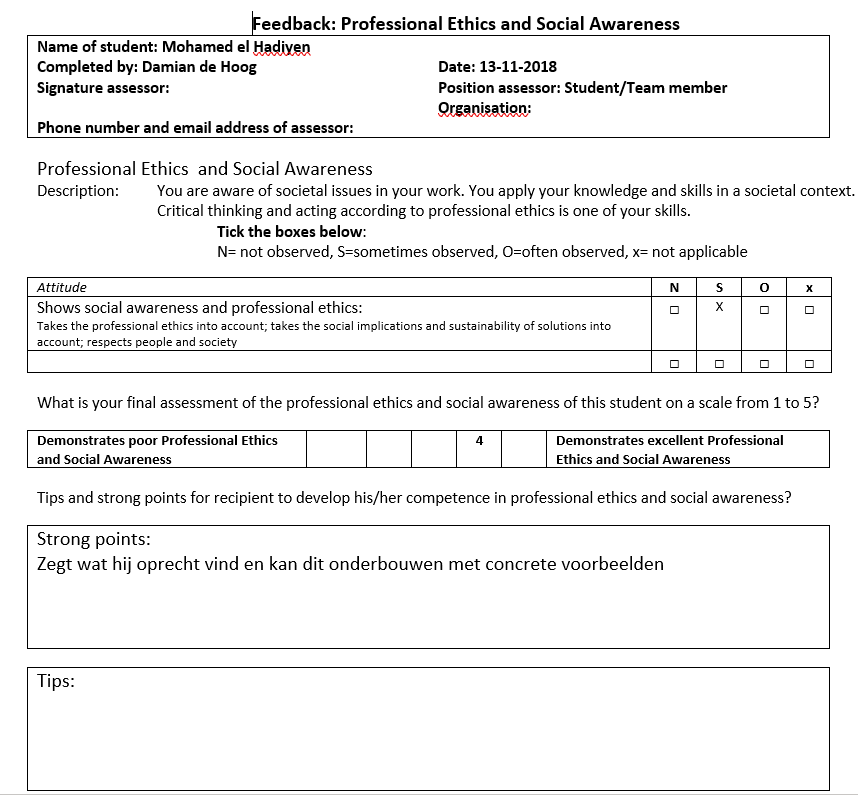
\includegraphics[width=\columnwidth]{ProfEthMohamed.PNG}\\
		\caption{Professional Ethics feedback Mohamed by Damian}
	\end{figure}
	\begin{figure}[p!]
		\centering
		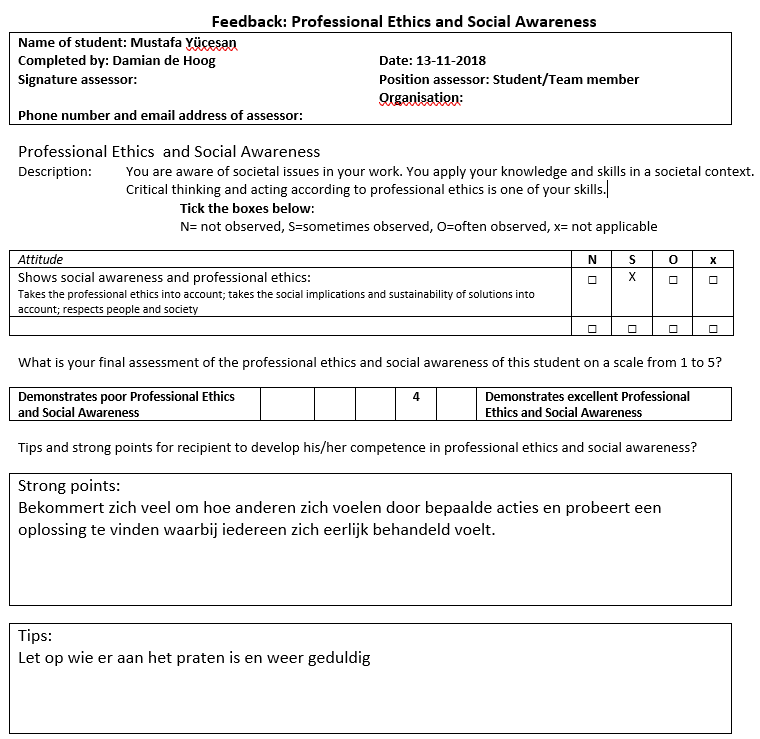
\includegraphics[width=\columnwidth]{ProfEthMustafa.PNG}\\
		\caption{Professional Ethics feedback Mustafa by Damian}
	\end{figure}
	\begin{figure}[p!]
		\centering
		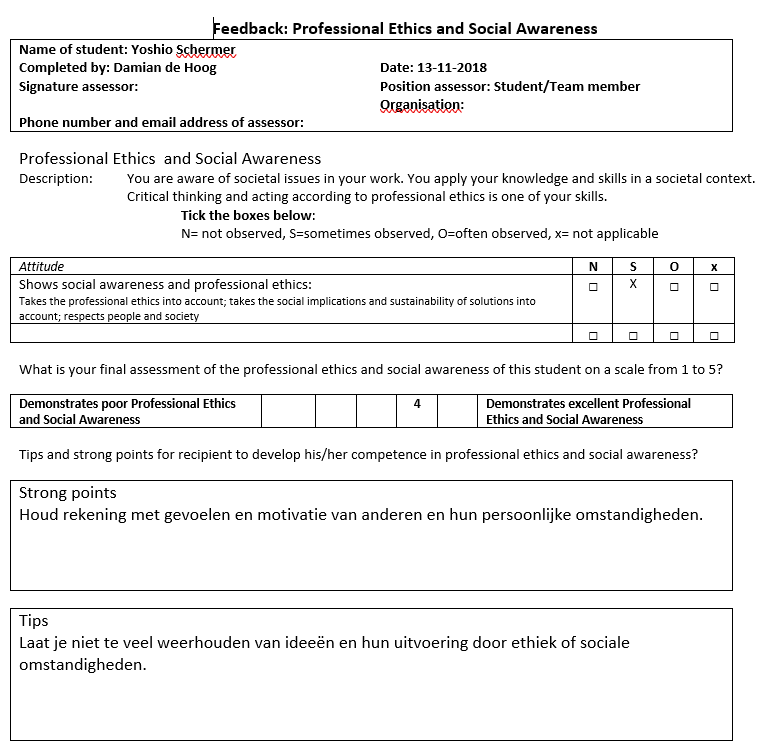
\includegraphics[width=\columnwidth]{ProfEthYoshio.PNG}\\
		\caption{Professional Ethics feedback Yoshio by Damian}
	\end{figure}
	\begin{figure}[p!]
		\centering
		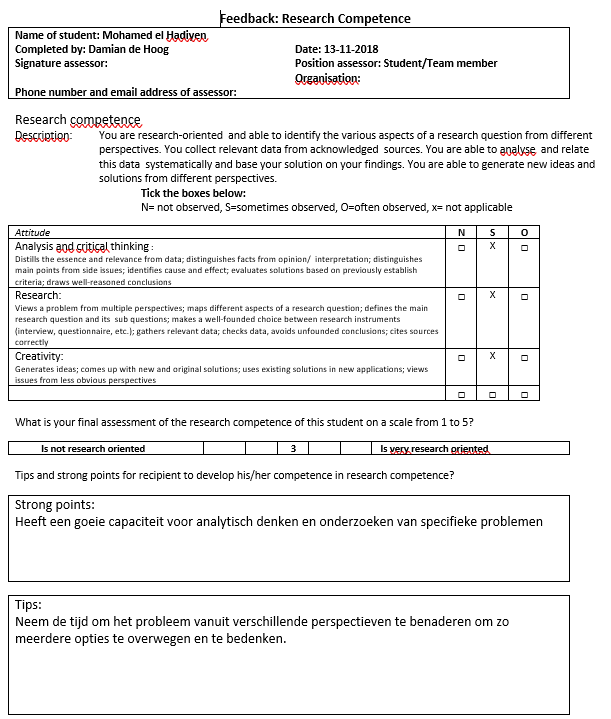
\includegraphics[width=\columnwidth]{ResSklMohamed.PNG}\\
		\caption{Research competence feedback Mohamed by Damian}
	\end{figure}
	\begin{figure}[p!]
		\centering
		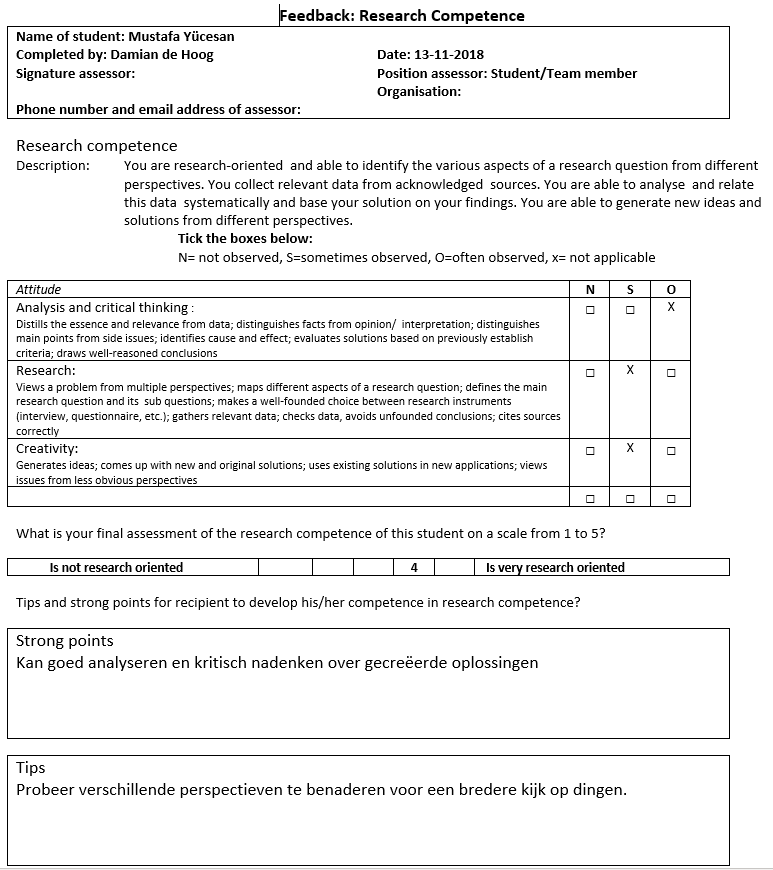
\includegraphics[width=\columnwidth]{ResSklMustafa.PNG}\\
		\caption{Research competence feedback Mustafa by Damian}
	\end{figure}
	\begin{figure}[p!]
		\centering
		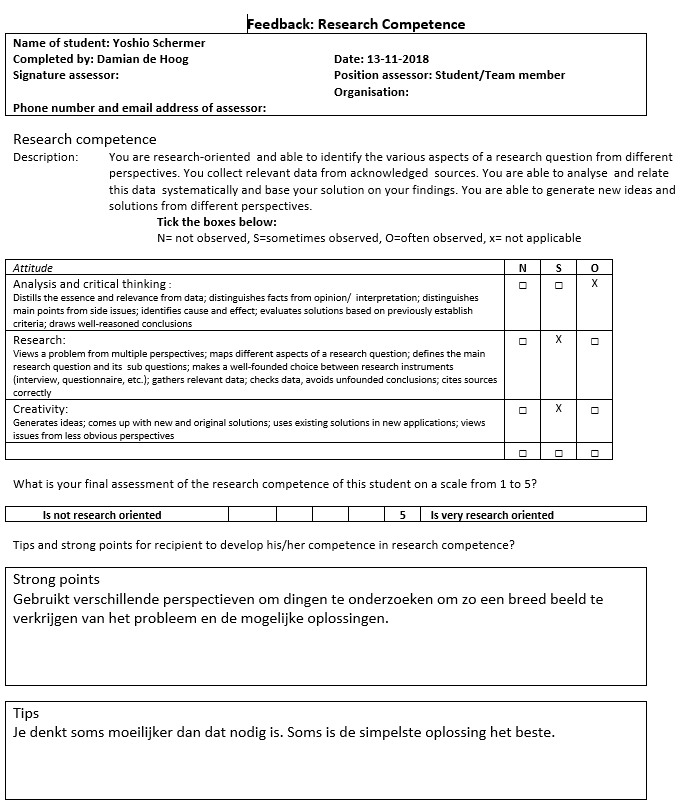
\includegraphics[width=\columnwidth]{ResSklYoshio.PNG}\\
		\caption{Research competence feedback Yoshio by Damian}
	\end{figure}
	\begin{figure}[p!]
		\centering
		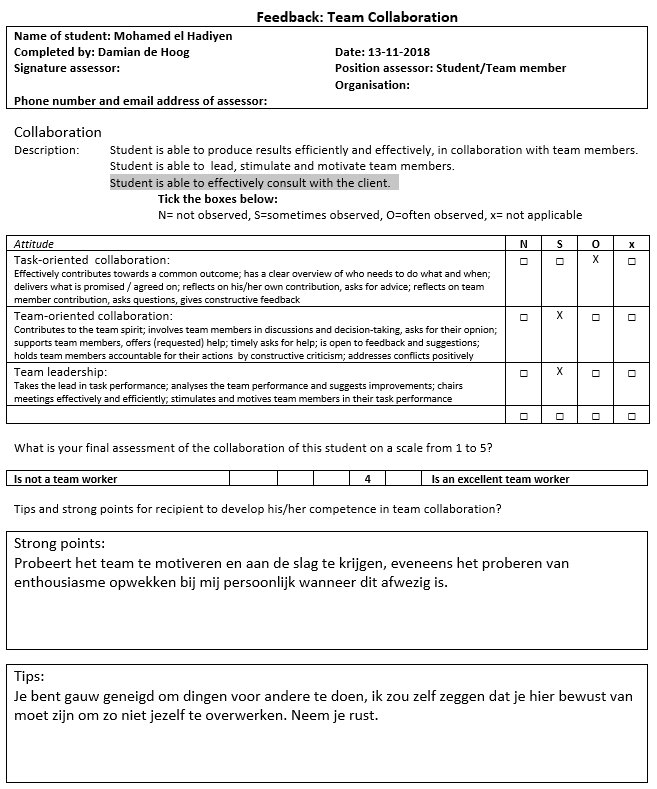
\includegraphics[width=\columnwidth]{CoopMohamed.PNG}\\
		\caption{Team Collaboration feedback Mohamed by Damian}
	\end{figure}
	\begin{figure}[p!]
		\centering
		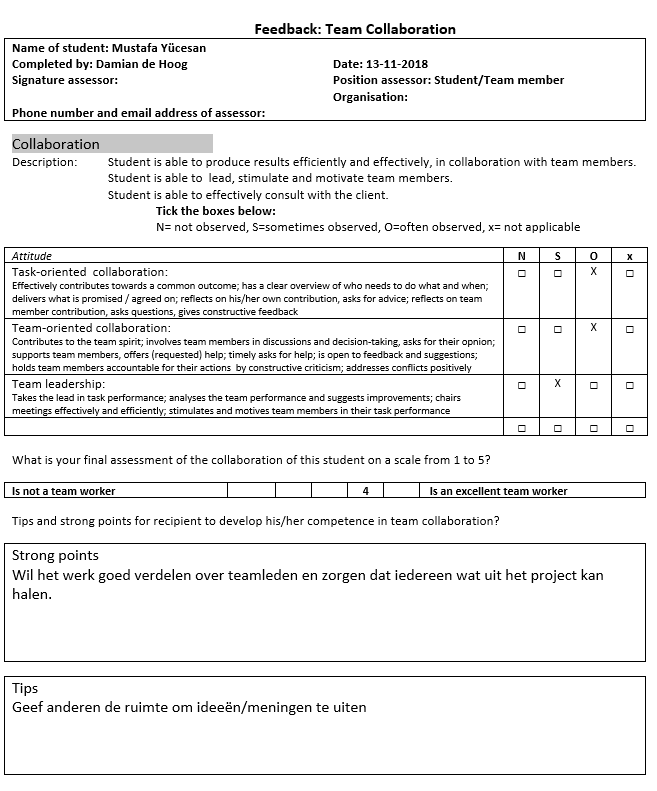
\includegraphics[width=\columnwidth]{CoopMustafa.PNG}\\
		\caption{Team Collaboration feedback Mustafa by Damian}
	\end{figure}
	\begin{figure}[p!]
		\centering
		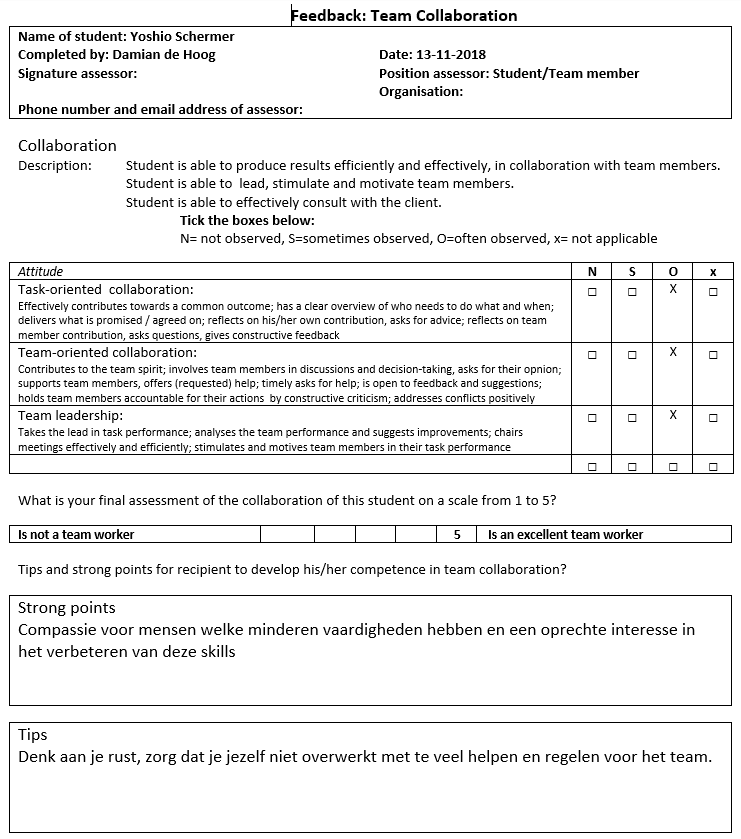
\includegraphics[width=\columnwidth]{CoopYoshio.PNG}\\
		\caption{Team Collaboration feedback Yoshio by Damian}
	\end{figure}
	\begin{figure}[p!]
		\centering
		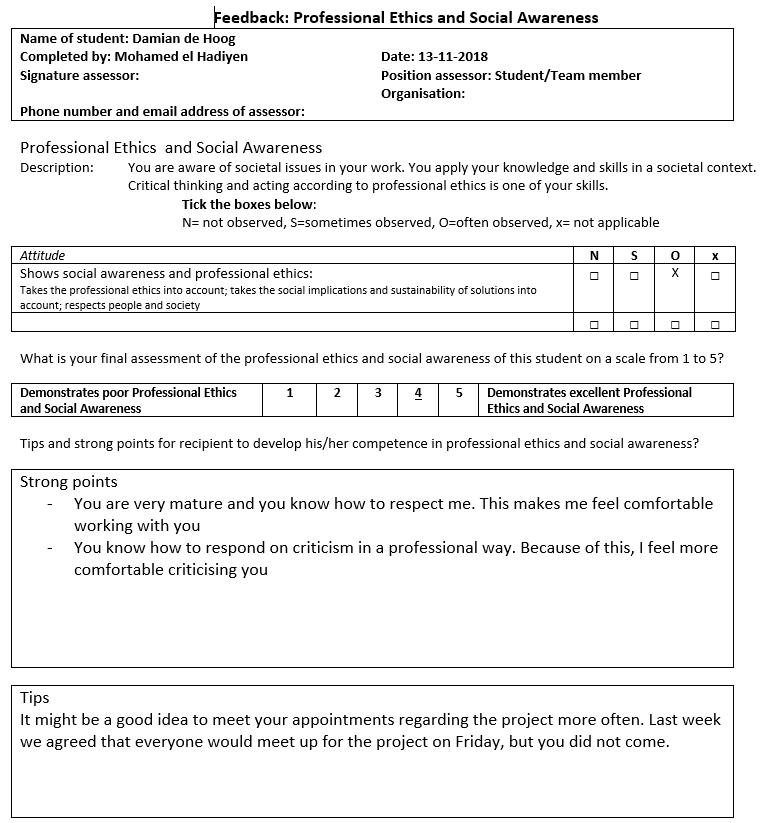
\includegraphics[width=\columnwidth]{ProfEthDamian1.PNG}\\
		\caption{Professional Ethics feedback Damian by Mohamed}
	\end{figure}
	\begin{figure}[p!]
		\centering
		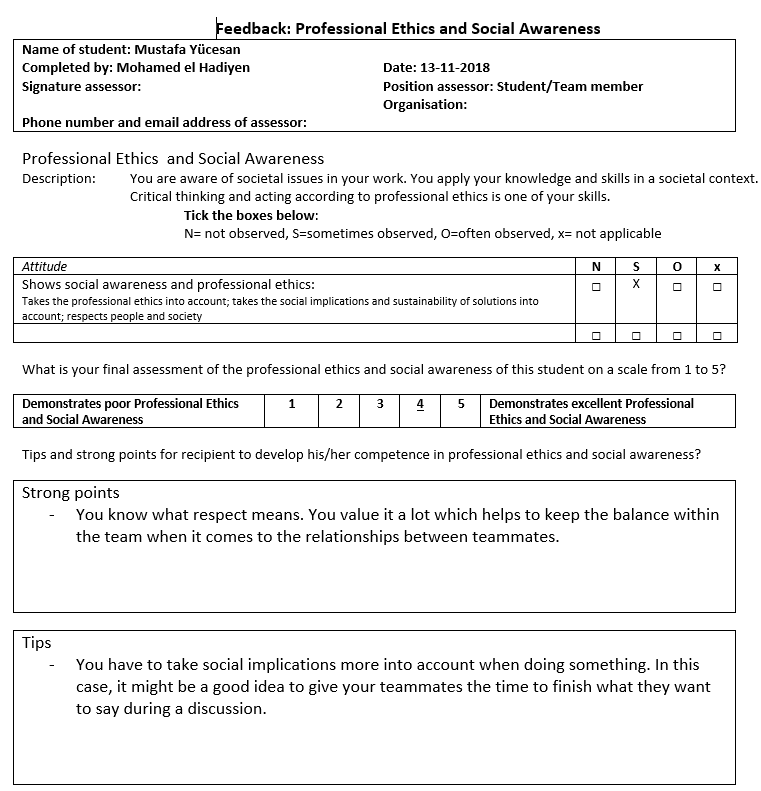
\includegraphics[width=\columnwidth]{ProfEthMustafa1.PNG}\\
		\caption{Professional Ethics feedback Mustafa by Mohamed}
	\end{figure}
	\begin{figure}[p!]
		\centering
		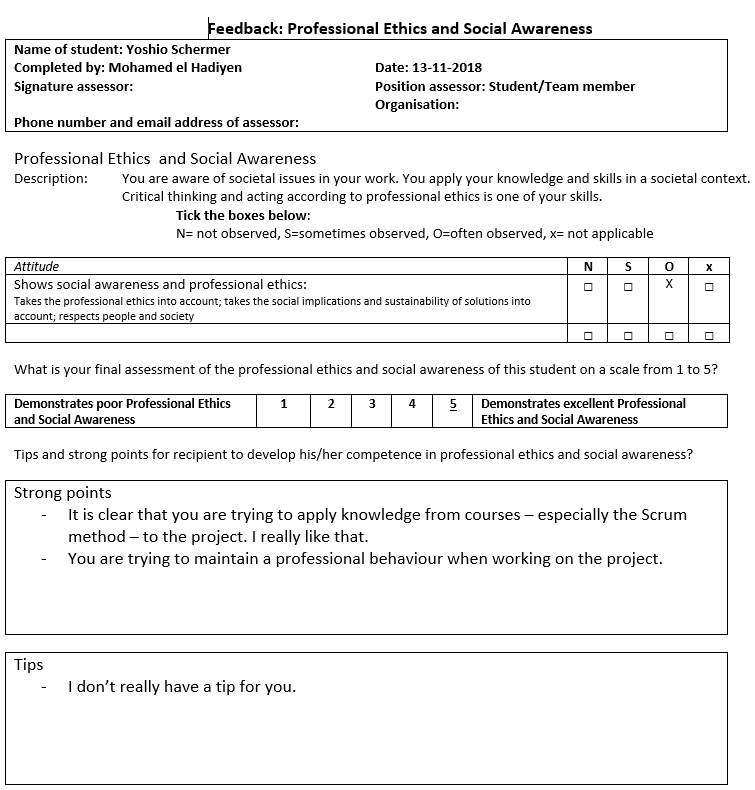
\includegraphics[width=\columnwidth]{ProfEthYoshio1.PNG}\\
		\caption{Professional Ethics feedback Yoshio by Mohamed}
	\end{figure}
	\begin{figure}[p!]
		\centering
		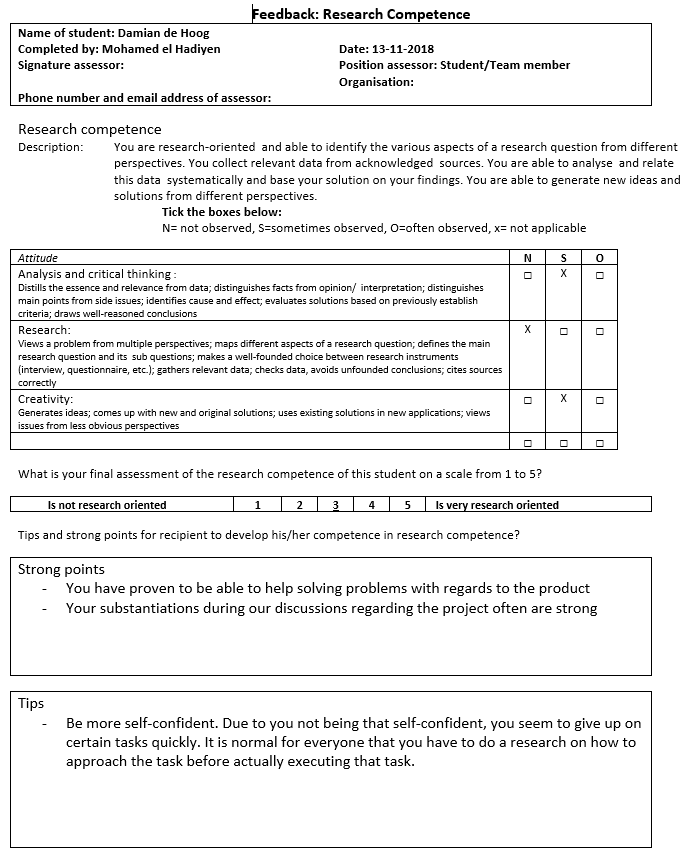
\includegraphics[width=\columnwidth]{ResSklDamian1.PNG}\\
		\caption{Research competence feedback Damian by Mohamed}
	\end{figure}
	\begin{figure}[p!]
		\centering
		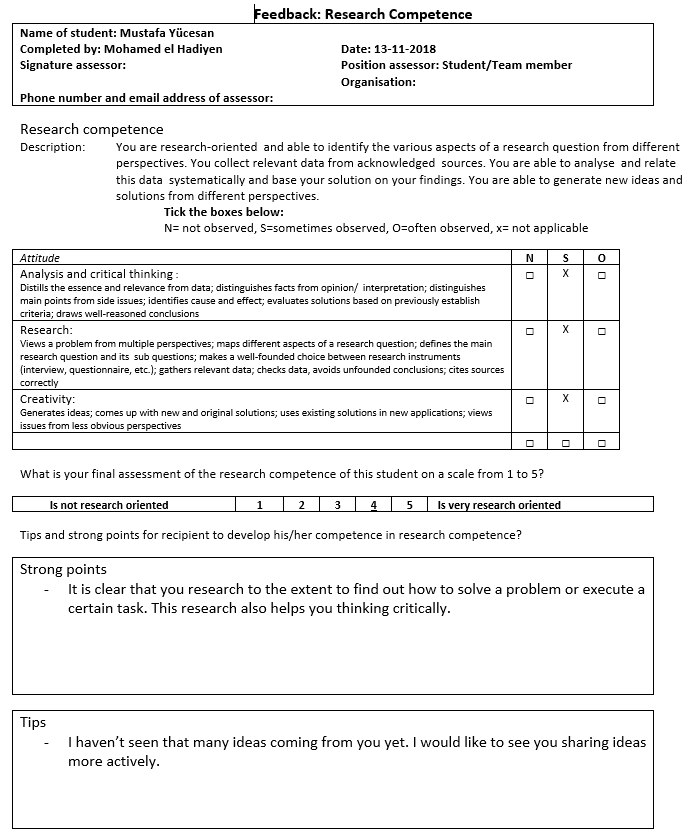
\includegraphics[width=\columnwidth]{ResSklMustafa1.PNG}\\
		\caption{Research competence feedback Mustafa by Mohamed}
	\end{figure}
	\begin{figure}[p!]
		\centering
		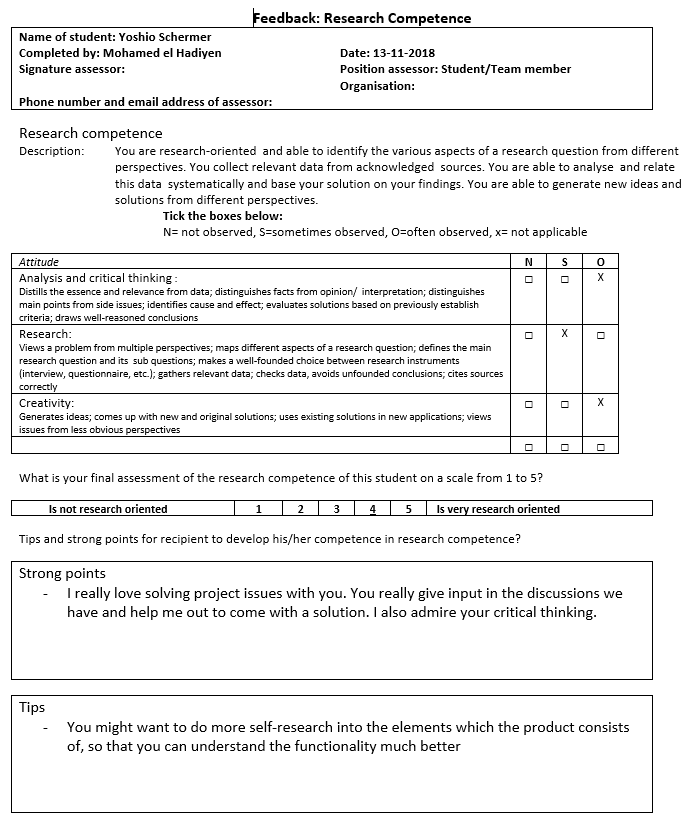
\includegraphics[width=\columnwidth]{ResSklYoshio1.PNG}\\
		\caption{Research competence feedback Yoshio by Mohamed}
	\end{figure}
	\begin{figure}[p!]
		\centering
		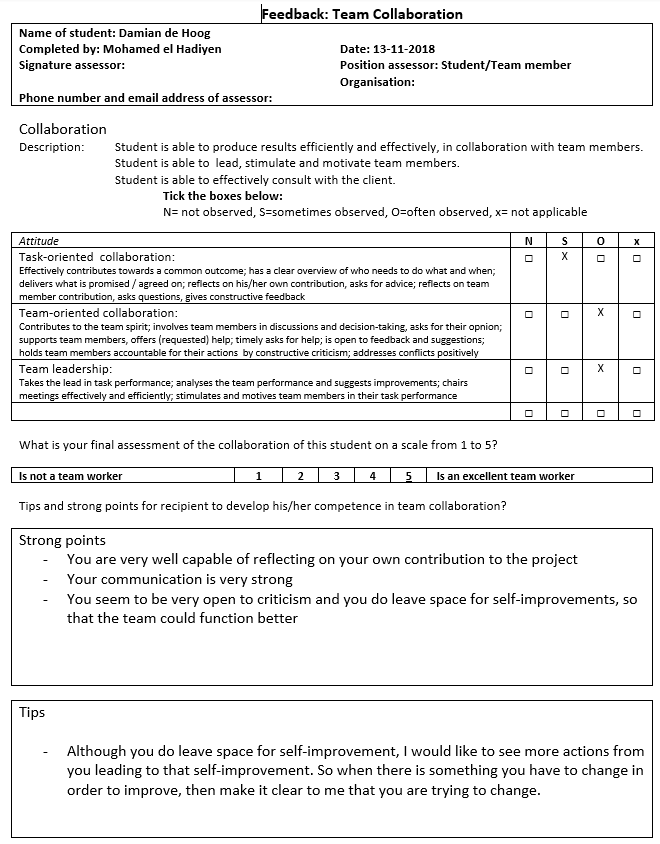
\includegraphics[width=\columnwidth]{CoopDamian1.PNG}\\
		\caption{Team Collaboration feedback Damian by Mohamed}
	\end{figure}
	\begin{figure}[p!]
		\centering
		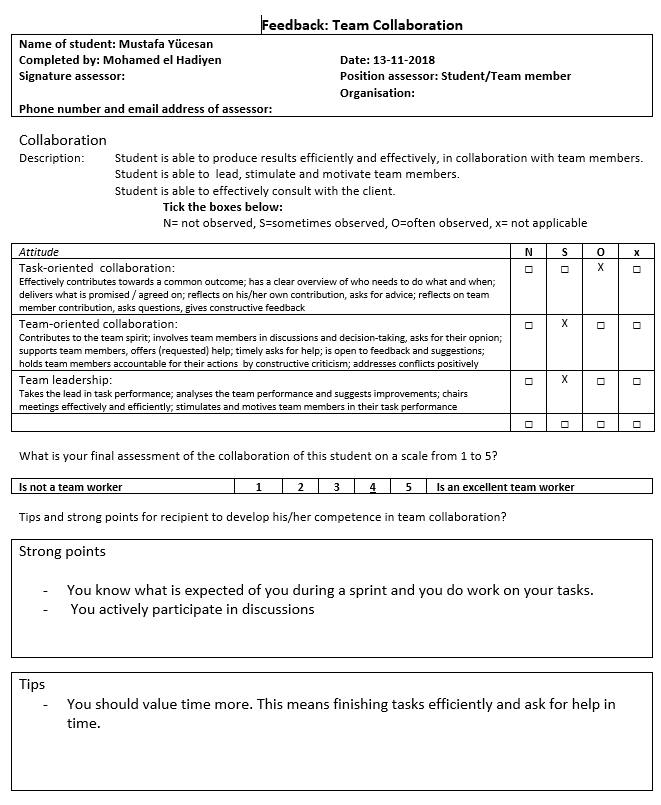
\includegraphics[width=\columnwidth]{CoopMustafa1.PNG}\\
		\caption{Team Collaboration feedback Mustafa by Mohamed}
	\end{figure}
	\begin{figure}[p!]
		\centering
		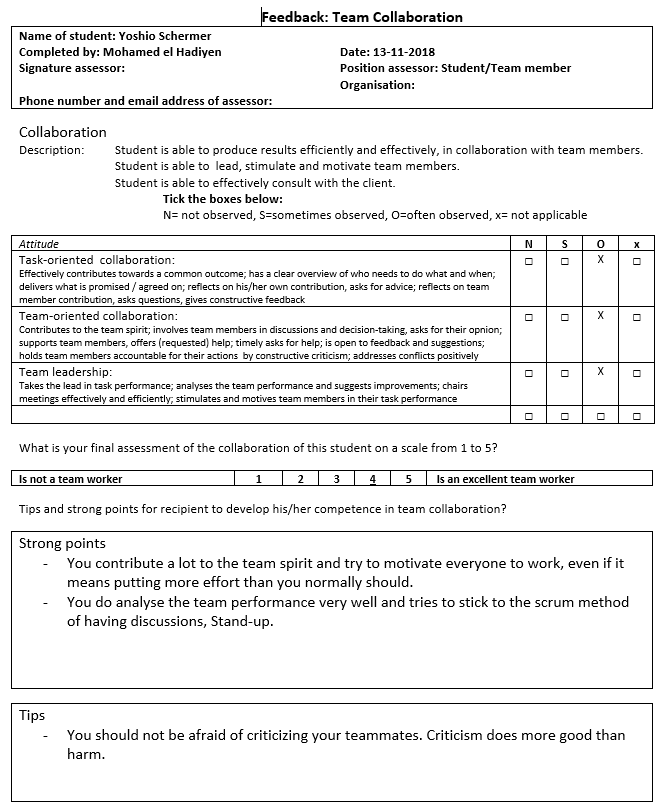
\includegraphics[width=\columnwidth]{CoopYoshio1.PNG}\\
		\caption{Team Collaboration feedback Yoshio by Mohamed}
	\end{figure}
	\begin{figure}[p!]
		\centering
		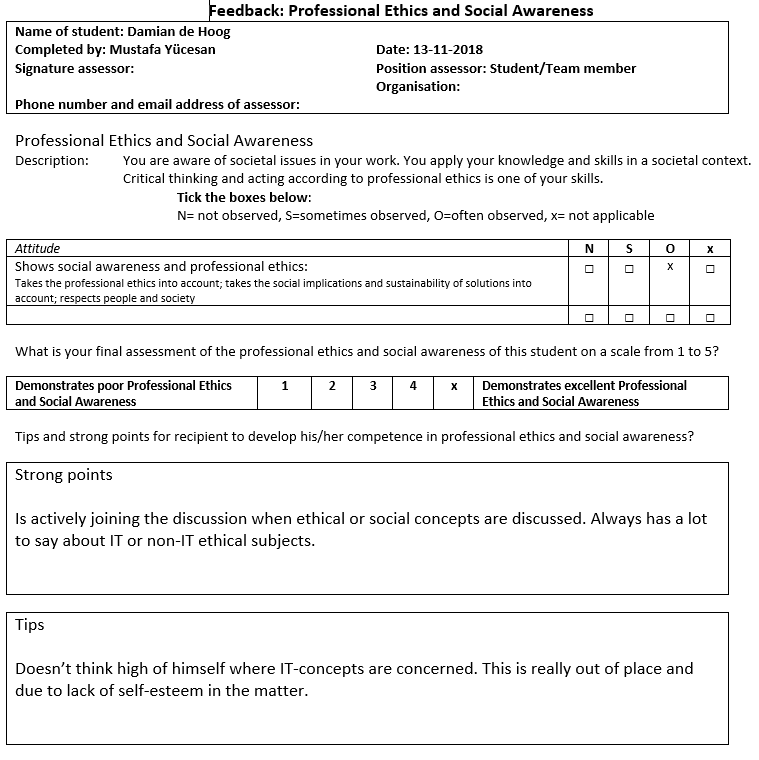
\includegraphics[width=\columnwidth]{ProfEthDamian2.PNG}\\
		\caption{Professional Ethics feedback Damian by Mustafa}
	\end{figure}
	\begin{figure}[p!]
		\centering
		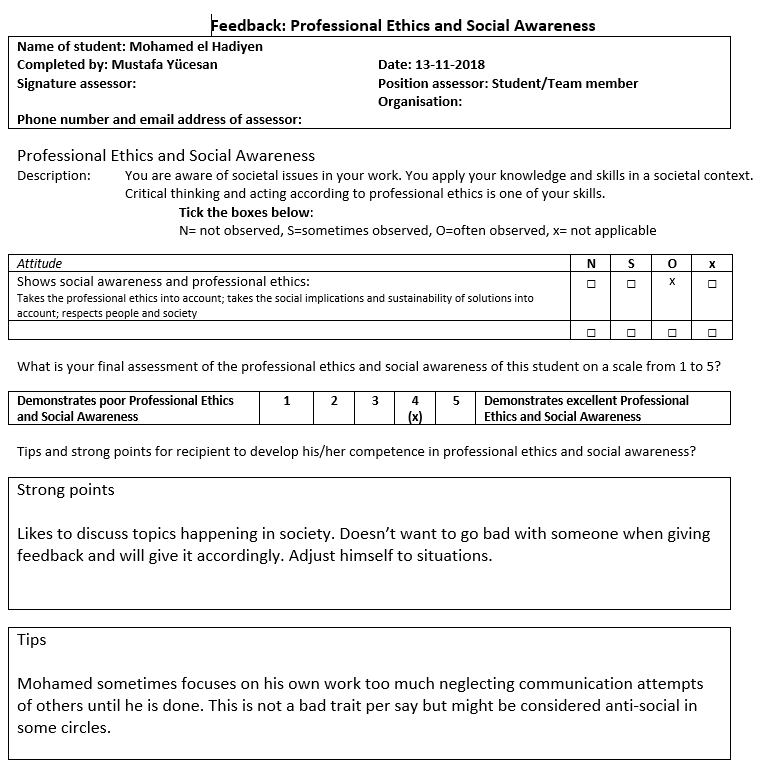
\includegraphics[width=\columnwidth]{ProfEthMohamed2.PNG}\\
		\caption{Professional Ethics feedback Mohamed by Mustafa}
	\end{figure}
	\begin{figure}[p!]
		\centering
		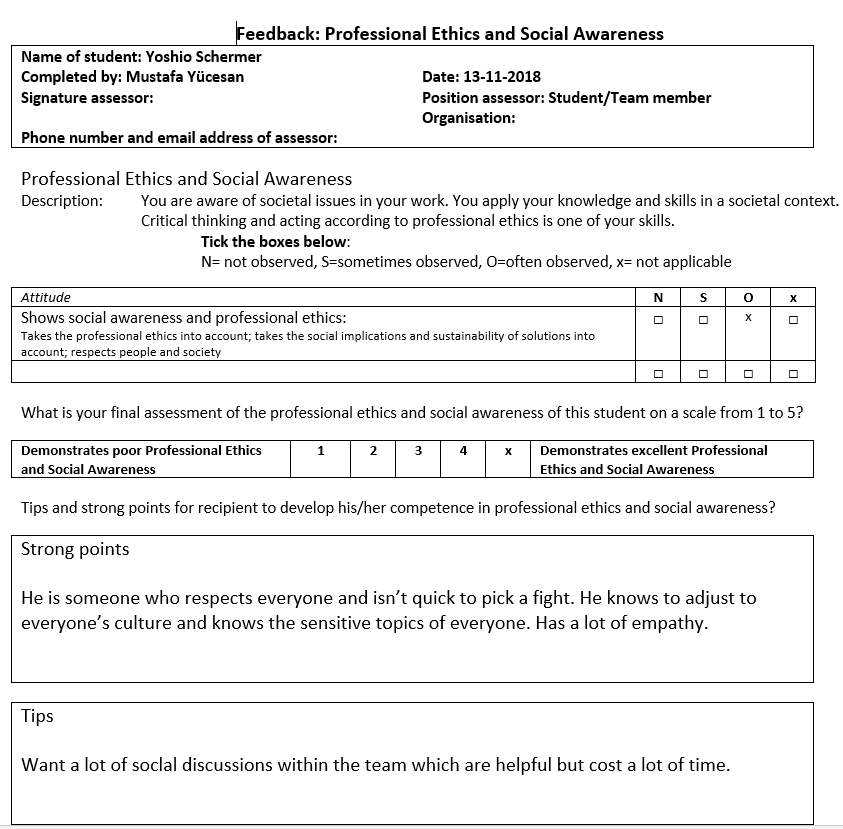
\includegraphics[width=\columnwidth]{ProfEthYoshio2.PNG}\\
		\caption{Professional Ethics feedback Yoshio by Mustafa}
	\end{figure}
	\begin{figure}[p!]
		\centering
		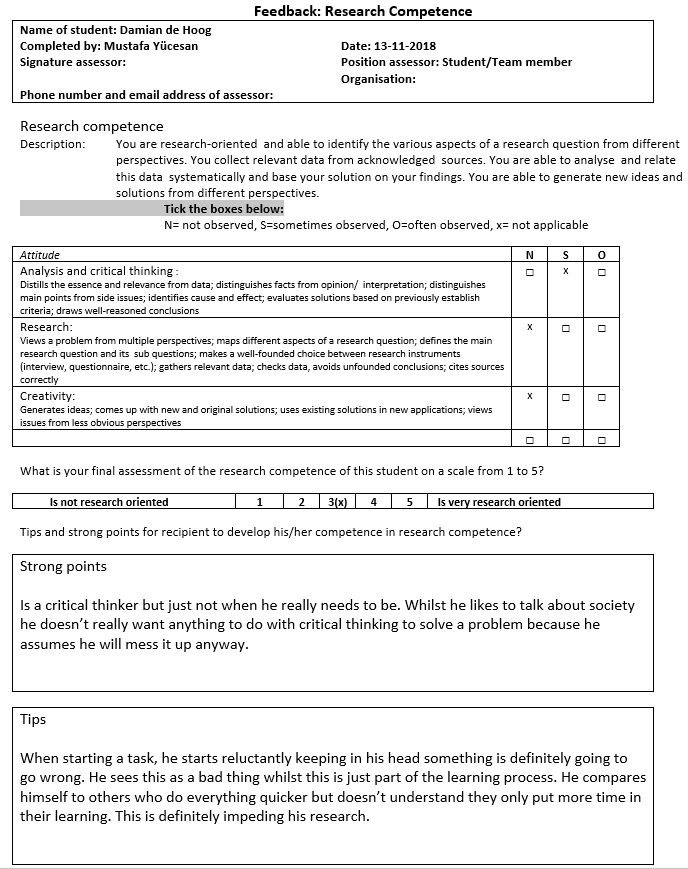
\includegraphics[width=\columnwidth]{ResSklDamian2.PNG}\\
		\caption{Research competence feedback Damian by Mustafa}
	\end{figure}
	\begin{figure}[p!]
		\centering
		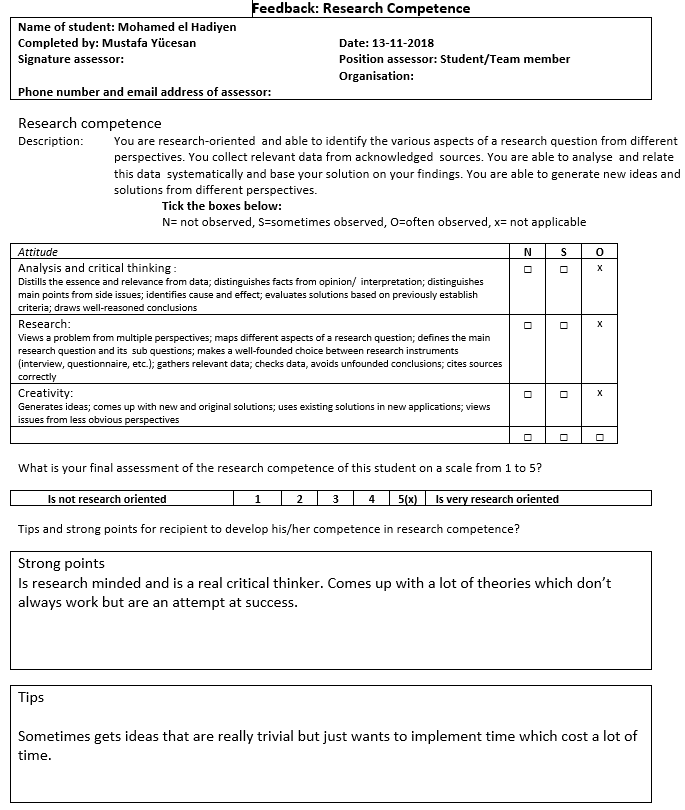
\includegraphics[width=\columnwidth]{ResSklMohamed2.PNG}\\
		\caption{Research competence feedback Mohamed by Mustafa}
	\end{figure}
	\begin{figure}[p!]
		\centering
		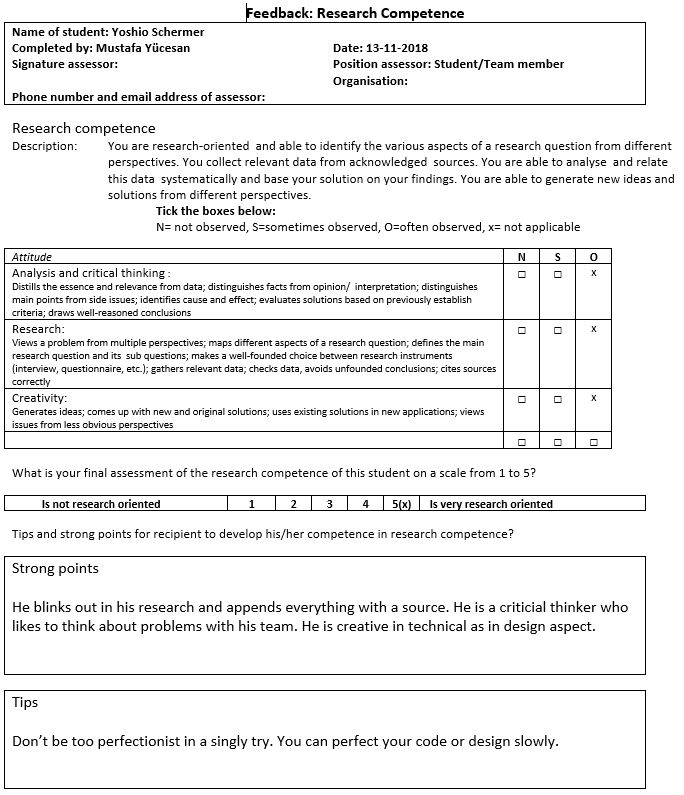
\includegraphics[width=\columnwidth]{ResSklYoshio2.PNG}\\
		\caption{Research competence feedback Yoshio by Mustafa}
	\end{figure}
	\begin{figure}[p!]
		\centering
		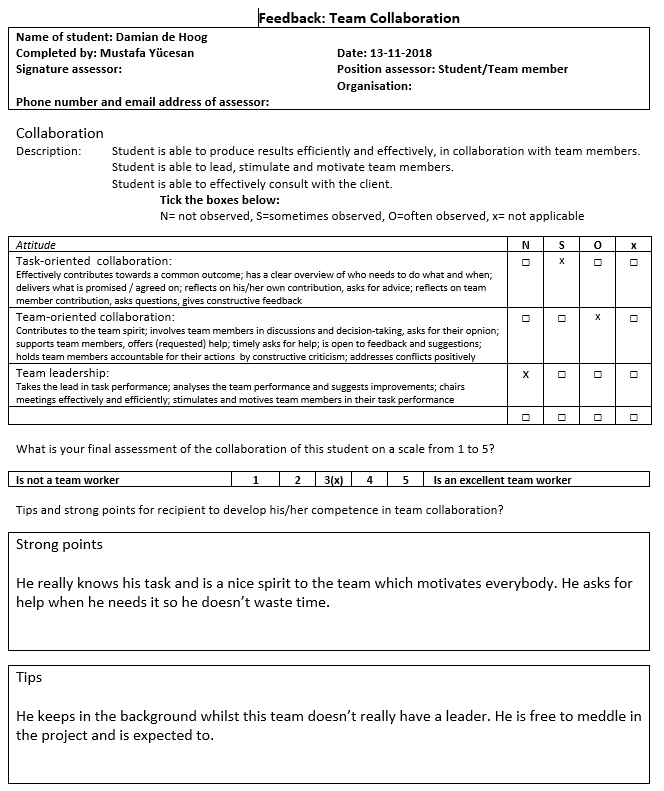
\includegraphics[width=\columnwidth]{CoopDamian2.PNG}\\
		\caption{Team Collaboration feedback Damian by Mustafa}
	\end{figure}
	\begin{figure}[p!]
		\centering
		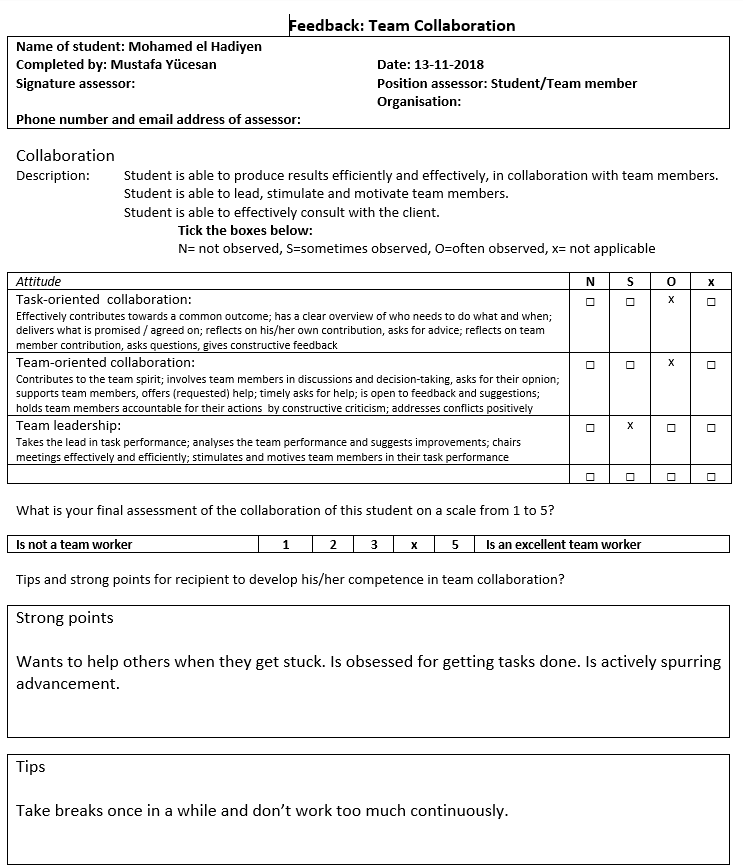
\includegraphics[width=\columnwidth]{CoopMohamed2.PNG}\\
		\caption{Team Collaboration feedback Mohamed by Mustafa}
	\end{figure}
	\begin{figure}[p!]
		\centering
		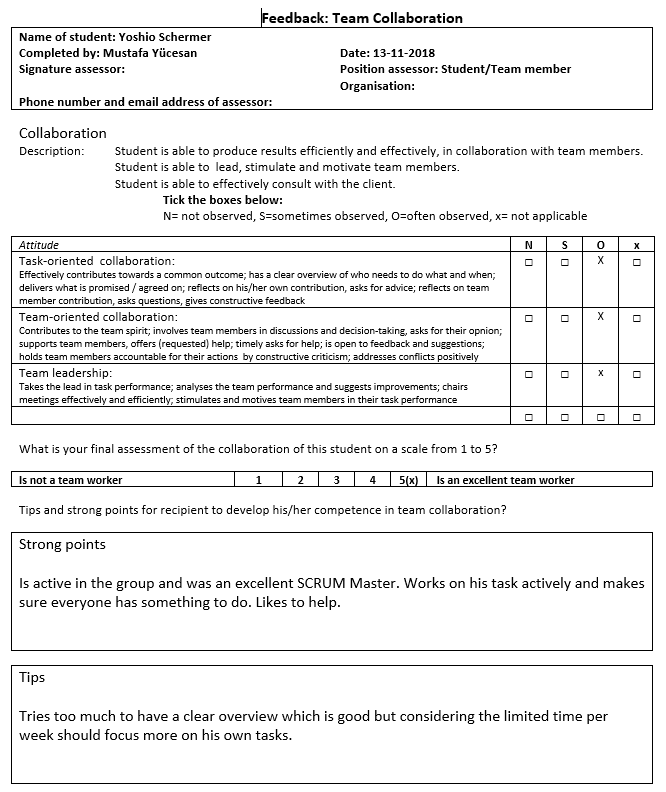
\includegraphics[width=\columnwidth]{CoopYoshio2.PNG}\\
		\caption{Team Collaboration feedback Yoshio by Mustafa}
	\end{figure}
	\begin{figure}[p!]
		\centering
		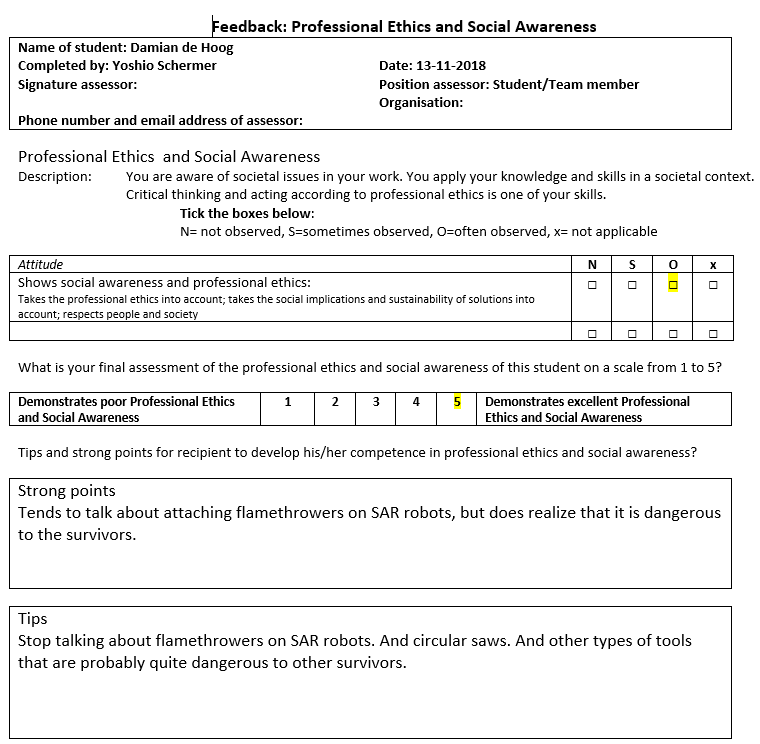
\includegraphics[width=\columnwidth]{ProfEthDamian3.PNG}\\
		\caption{Professional Ethics feedback Damian by Yoshio}
	\end{figure}
	\begin{figure}[p!]
		\centering
		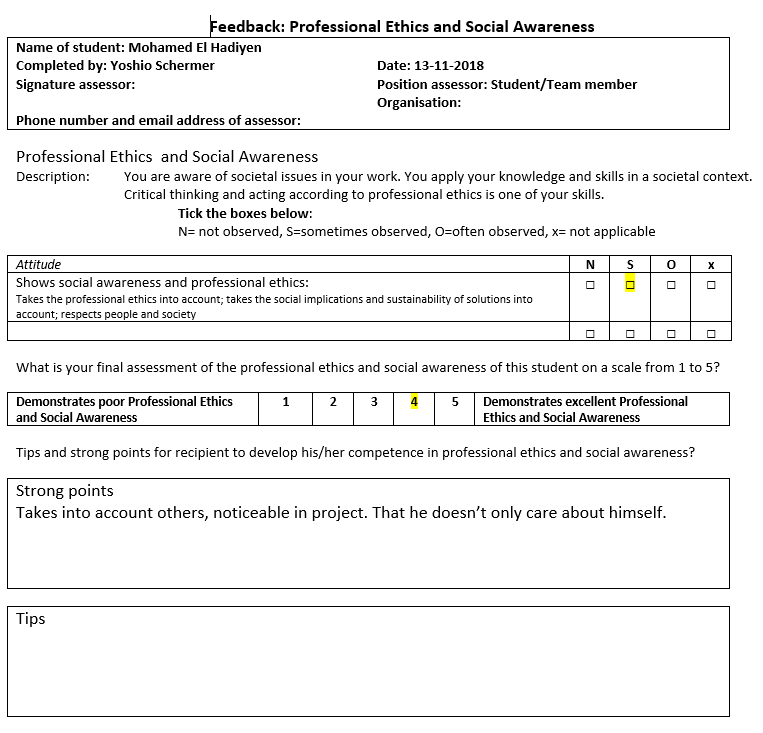
\includegraphics[width=\columnwidth]{ProfEthMohamed3.PNG}\\
		\caption{Professional Ethics feedback Mohamed by Yoshio}
	\end{figure}
	\begin{figure}[p!]
		\centering
		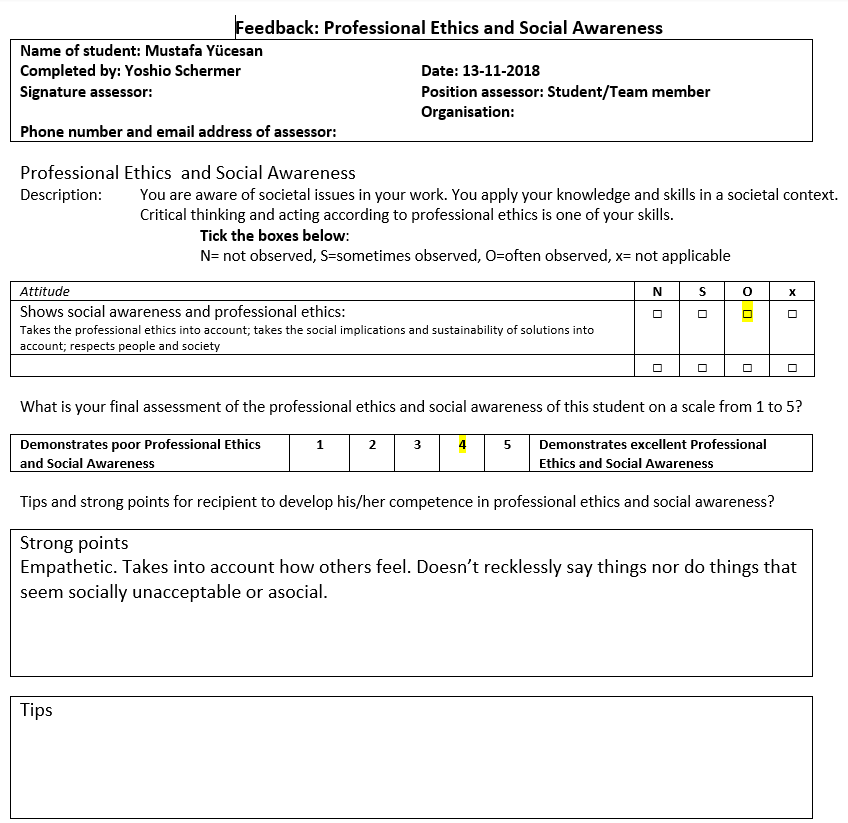
\includegraphics[width=\columnwidth]{ProfEthMustafa3.PNG}\\
		\caption{Professional Ethics feedback Mustafa by Yoshio}
	\end{figure}
	\begin{figure}[p!]
		\centering
		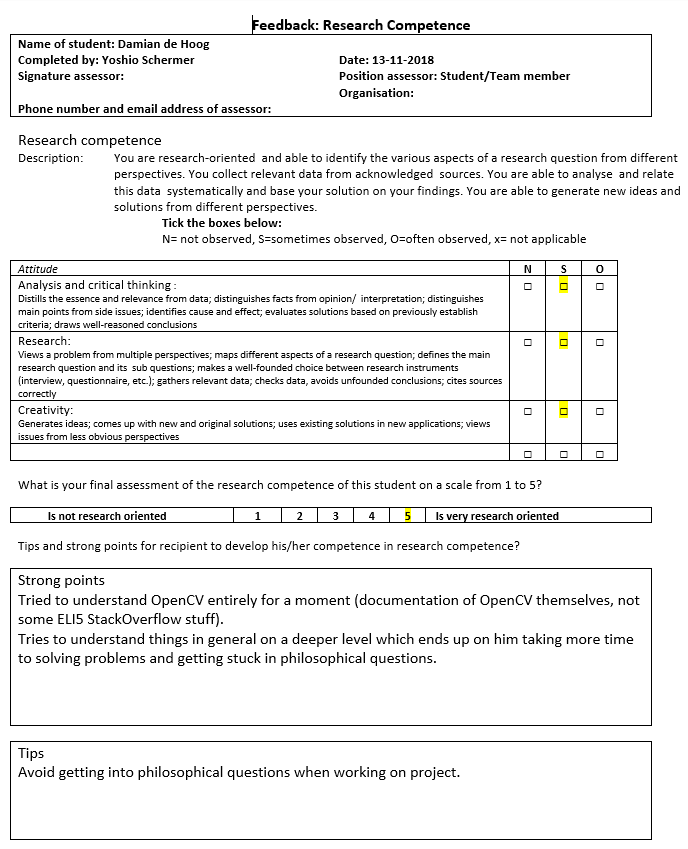
\includegraphics[width=\columnwidth]{ResSklDamian3.PNG}\\
		\caption{Research competence feedback Damian by Yoshio}
	\end{figure}
	\begin{figure}[p!]
		\centering
		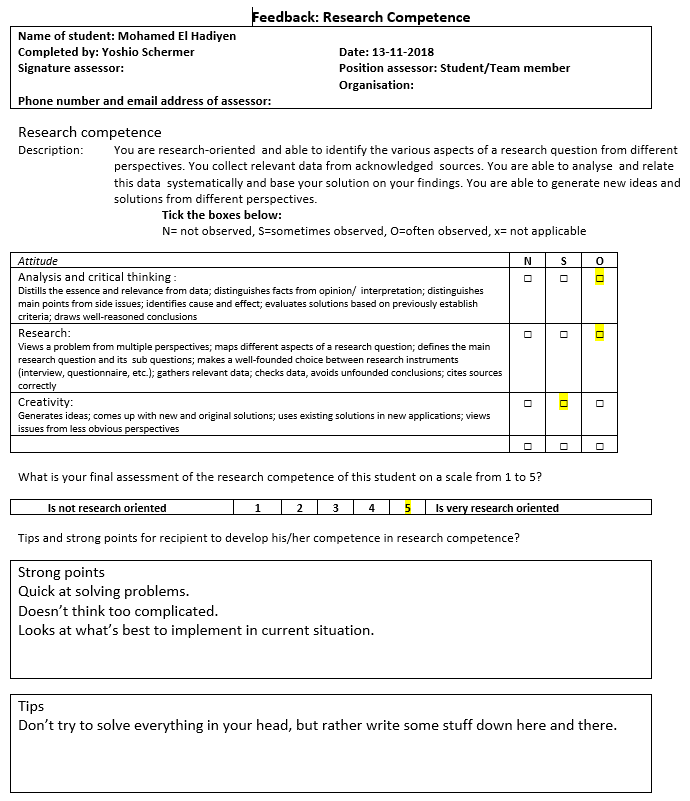
\includegraphics[width=\columnwidth]{ResSklMohamed3.PNG}\\
		\caption{Research competence feedback Mohamed by Yoshio}
	\end{figure}
	\begin{figure}[p!]
		\centering
		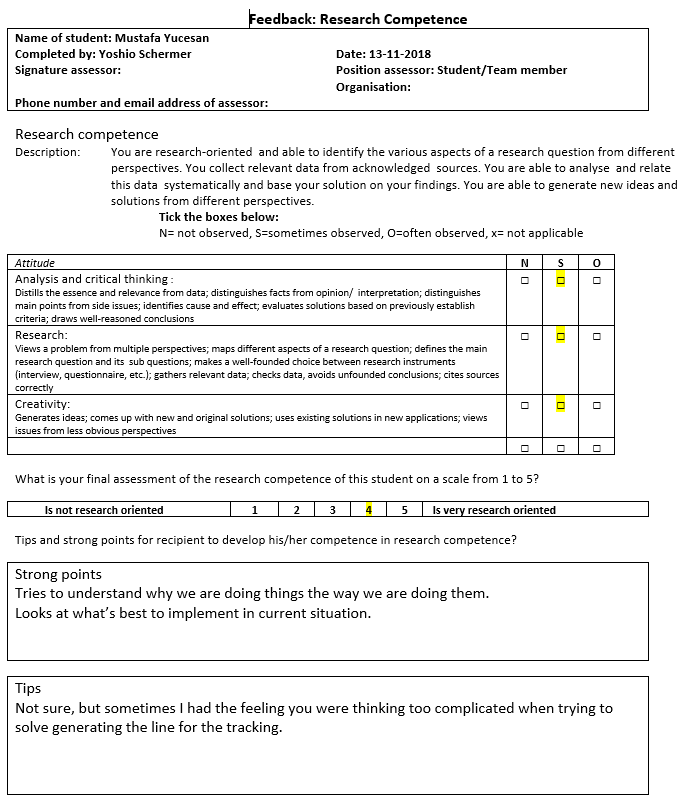
\includegraphics[width=\columnwidth]{ResSklMustafa3.PNG}\\
		\caption{Research competence feedback Mustafa by Yoshio}
	\end{figure}
	\begin{figure}[p!]
		\centering
		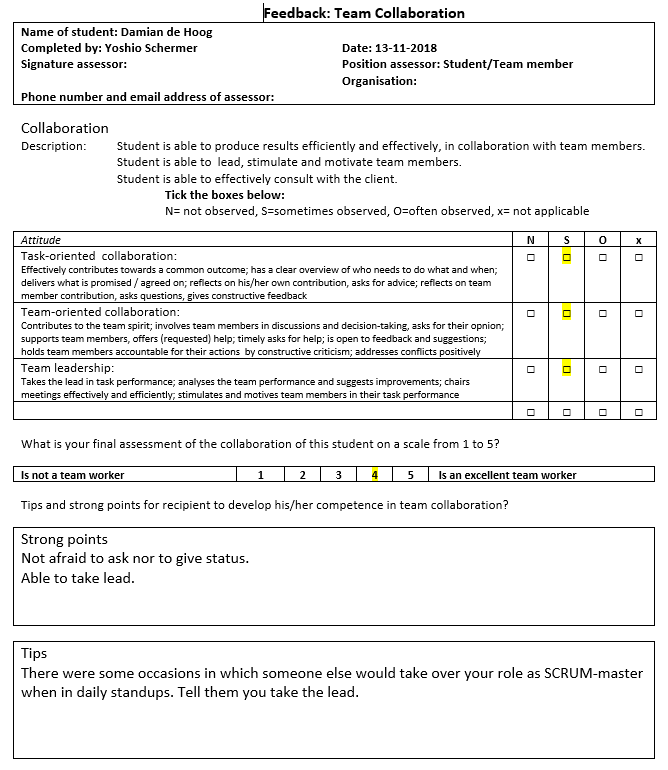
\includegraphics[width=\columnwidth]{CoopDamian3.PNG}\\
		\caption{Team Collaboration feedback Damian by Yoshio}
	\end{figure}
	\begin{figure}[p!]
		\centering
		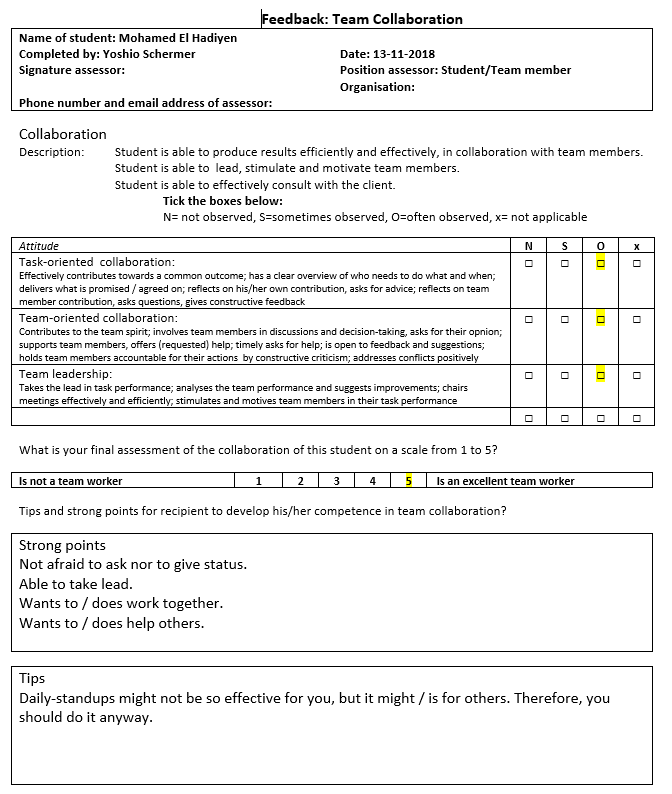
\includegraphics[width=\columnwidth]{CoopMohamed3.PNG}\\
		\caption{Team Collaboration feedback Mohamed by Yoshio}
	\end{figure}
	\begin{figure}[p!]
		\centering
		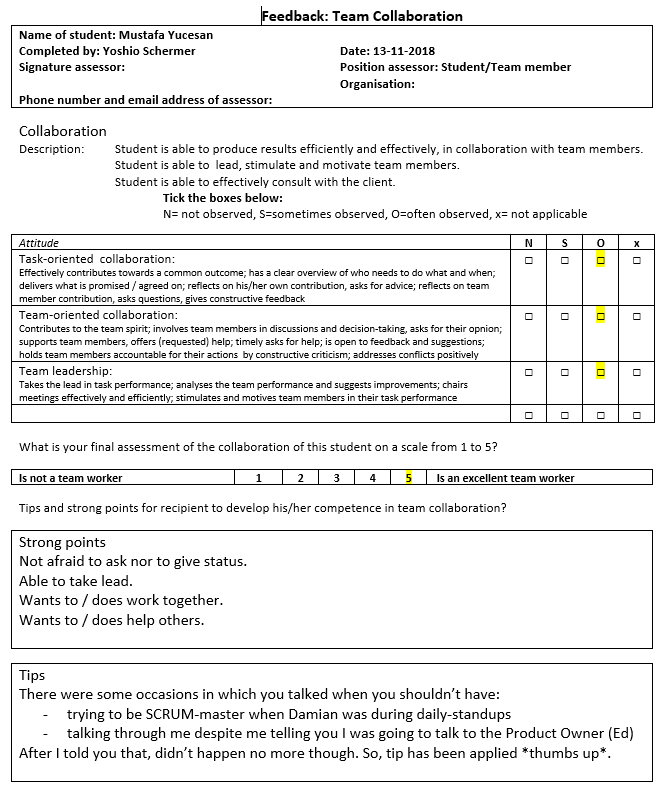
\includegraphics[width=\columnwidth]{CoopMustafa3.PNG}\\
		\caption{Team Collaboration feedback Mustafa by Yoshio}
	\end{figure}
\end{document}	